\chapter{MRI\label{chapter:mri}}
\lhead{MRI}
\begin{refsection}
\chapterauthor{Andreas Linggi, Daniel Monti und Nicol\'as Rom\'an L"uthold}

\printbibliography[heading=subbibliography]
\end{refsection}

\begin{minipage}{0.36\textwidth}
	\begin{figure}[H]
		\centering
		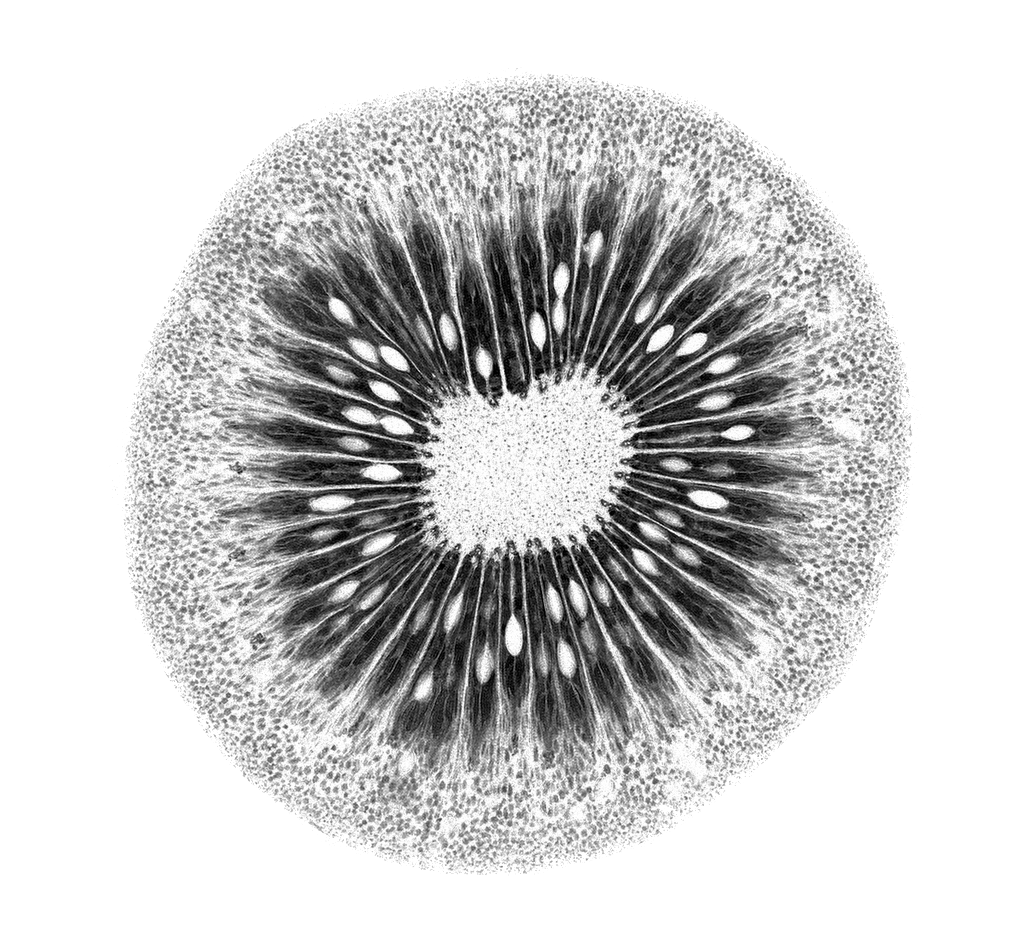
\includegraphics[height = 4.5cm]{./mri/pic/Kiwi.png}
		\caption{MRI einer Kiwi \cite{skript:mri:kiwi}}
		\label{mri:abb:kiwi}
	\end{figure}
\end{minipage}
\begin{minipage}{0.64\textwidth}
	\begin{figure}[H]
		\centering
		\includegraphics[height = 4.5cm]{./mri/pic/pinaple.png}
		\caption{MRI einer Ananas \cite{skript:mri:pinaple}}
		\label{mri:abb:ananas}
	\end{figure}
\end{minipage}
\vspace*{5mm}



{\parindent 0pt % this is a hack to remove the indentation from the paragraph
                % normally, the first paragraph is not indented, but this
                % paragraph is preceded by an image, which makes it 
                % technically not the first paragraph
MRI }(Magnetic Resonance Imaging) ist ein Verfahren, in dem die
\index{MRI}
Protonendichte von dreidimensionalen Objekten gemessen werden und
als Bilder dargestellt werden kann. Dazu werden die magnetisches
Eigenschaften von Protonen genutzt, um sie in Resonanz zu bringen.
Im Englischen ist dieses unter dem Begriff NMR (Nuclear Magnetic
Resonance) bekannt.
\index{NMR}
\index{Nuclear Magnetic Resonance}
In den folgenden Kapiteln wird gezeigt, wie die Protonendichte gemessen und wie sie als Bilder dargestellt werden kann. Es werden verschiedene Anwendungen vorgestellt und erkl"art.

\section{Klassisches Modell}
\rhead{Klassisches Modell}
In diesem Abschnitt soll das Prinzip des MRI mit Hilfe eines klassischen Modells des Verhaltens eines Protons im Magnetfeld erkl"art werden. Eine quantenmechanischen Beschreibung wird in Abschnitt \ref{sec:quant} gegeben. 

	\subsection{Protonen im Magnetfeld}
	
	Protonen k"onnen im klassischem Modell als rotierende Stabmagnete modelliert werden. Jedes dieser Magnete hat dadurch ein magnetisches Dipolmoment $\vec{\mu}$. Um das magnetischen Dipolmoment in einem Magnetfeld $\vec{B}$ zu drehen, ist eine Kraft n"otig, es muss Arbeit geleistet werden. Die Energie h"angt somit vom Winkel $\theta$ zwischen Magnetfeld und Dipolmoment ab gem"ass der Formel
\index{Dipolmoment}
\index{magnetisches Dipolmoment}
	\begin{equation}
		E_{\text{pot}}= -\vec{\mu} \cdot\vec{B} = -\mu B\cos\theta.
	\end{equation}
	Dabei ist jeder Winkel $\theta$ m"oglich. Mit zunehmendem Winkel $\theta$ nimmt auch die Energie zu bis $\theta = \pi$, danach nimmt die Energie wieder ab. 
%	Wie sich in Kapitel \ref{sec:quant} zeigen wird, ist der exakte Winkel f�r die weiteren Berechnungen nicht entscheidend.
	
	\subsection{Larmor-Pr"azession}
\index{Larmor-Pr"azession}	
	Bis jetzt wurde der Drehimpuls des Protons nicht ber"ucksichtigt. 
	Wenn sich nun ein Proton in einem Magnetfeld $\vec{B}$ befindet, versucht dieses den Drehimpuls auszurichten. Das Proton beginnt zu pr"azedieren.
	Diese Pr"azession heisst, nach dem irischen Physiker Joseph Larmor, Larmorpr"azession. Die Frequenz der Pr"azessionsbewegung wird Lamrorfrequenz $f_{\text{Larmor}}$ genannt \cite{wiki:larmorpraezession}. Sie ist abh"angig von der externen magnetischen Flussdichte $\vec{B_0}$ und von den magnetischen Dipolmoment. Bei einem Proton sind das Dipolmoment und der Drehimpuls gekoppelt. Dies f"uhrt zu folgenden Gleichung:
	\begin{equation}
	f_{\text{Larmor}} = \dfrac{\gamma B_0}{2\pi}\label{eq:larmorf}
	\end{equation}
	Das gyromagnetische Verh"altnis $\gamma$ variiert je nach Teilchenart. Im klassischen Modell ist dieses Verh"altnis eine Materialkonstante, die nicht aus klassischen Grundprinzipien hergeleitet werden kann.
\index{gyromagnetisches Verhaltnis@gyromagnetisches Verh\"altnis}
	
	Aus Gleichung \ref{eq:larmorf} ist erkennbar, dass die Larmorfrequenz nicht vom Winkel $\theta$ abh"angig ist.

	\begin{figure}
		\centering
		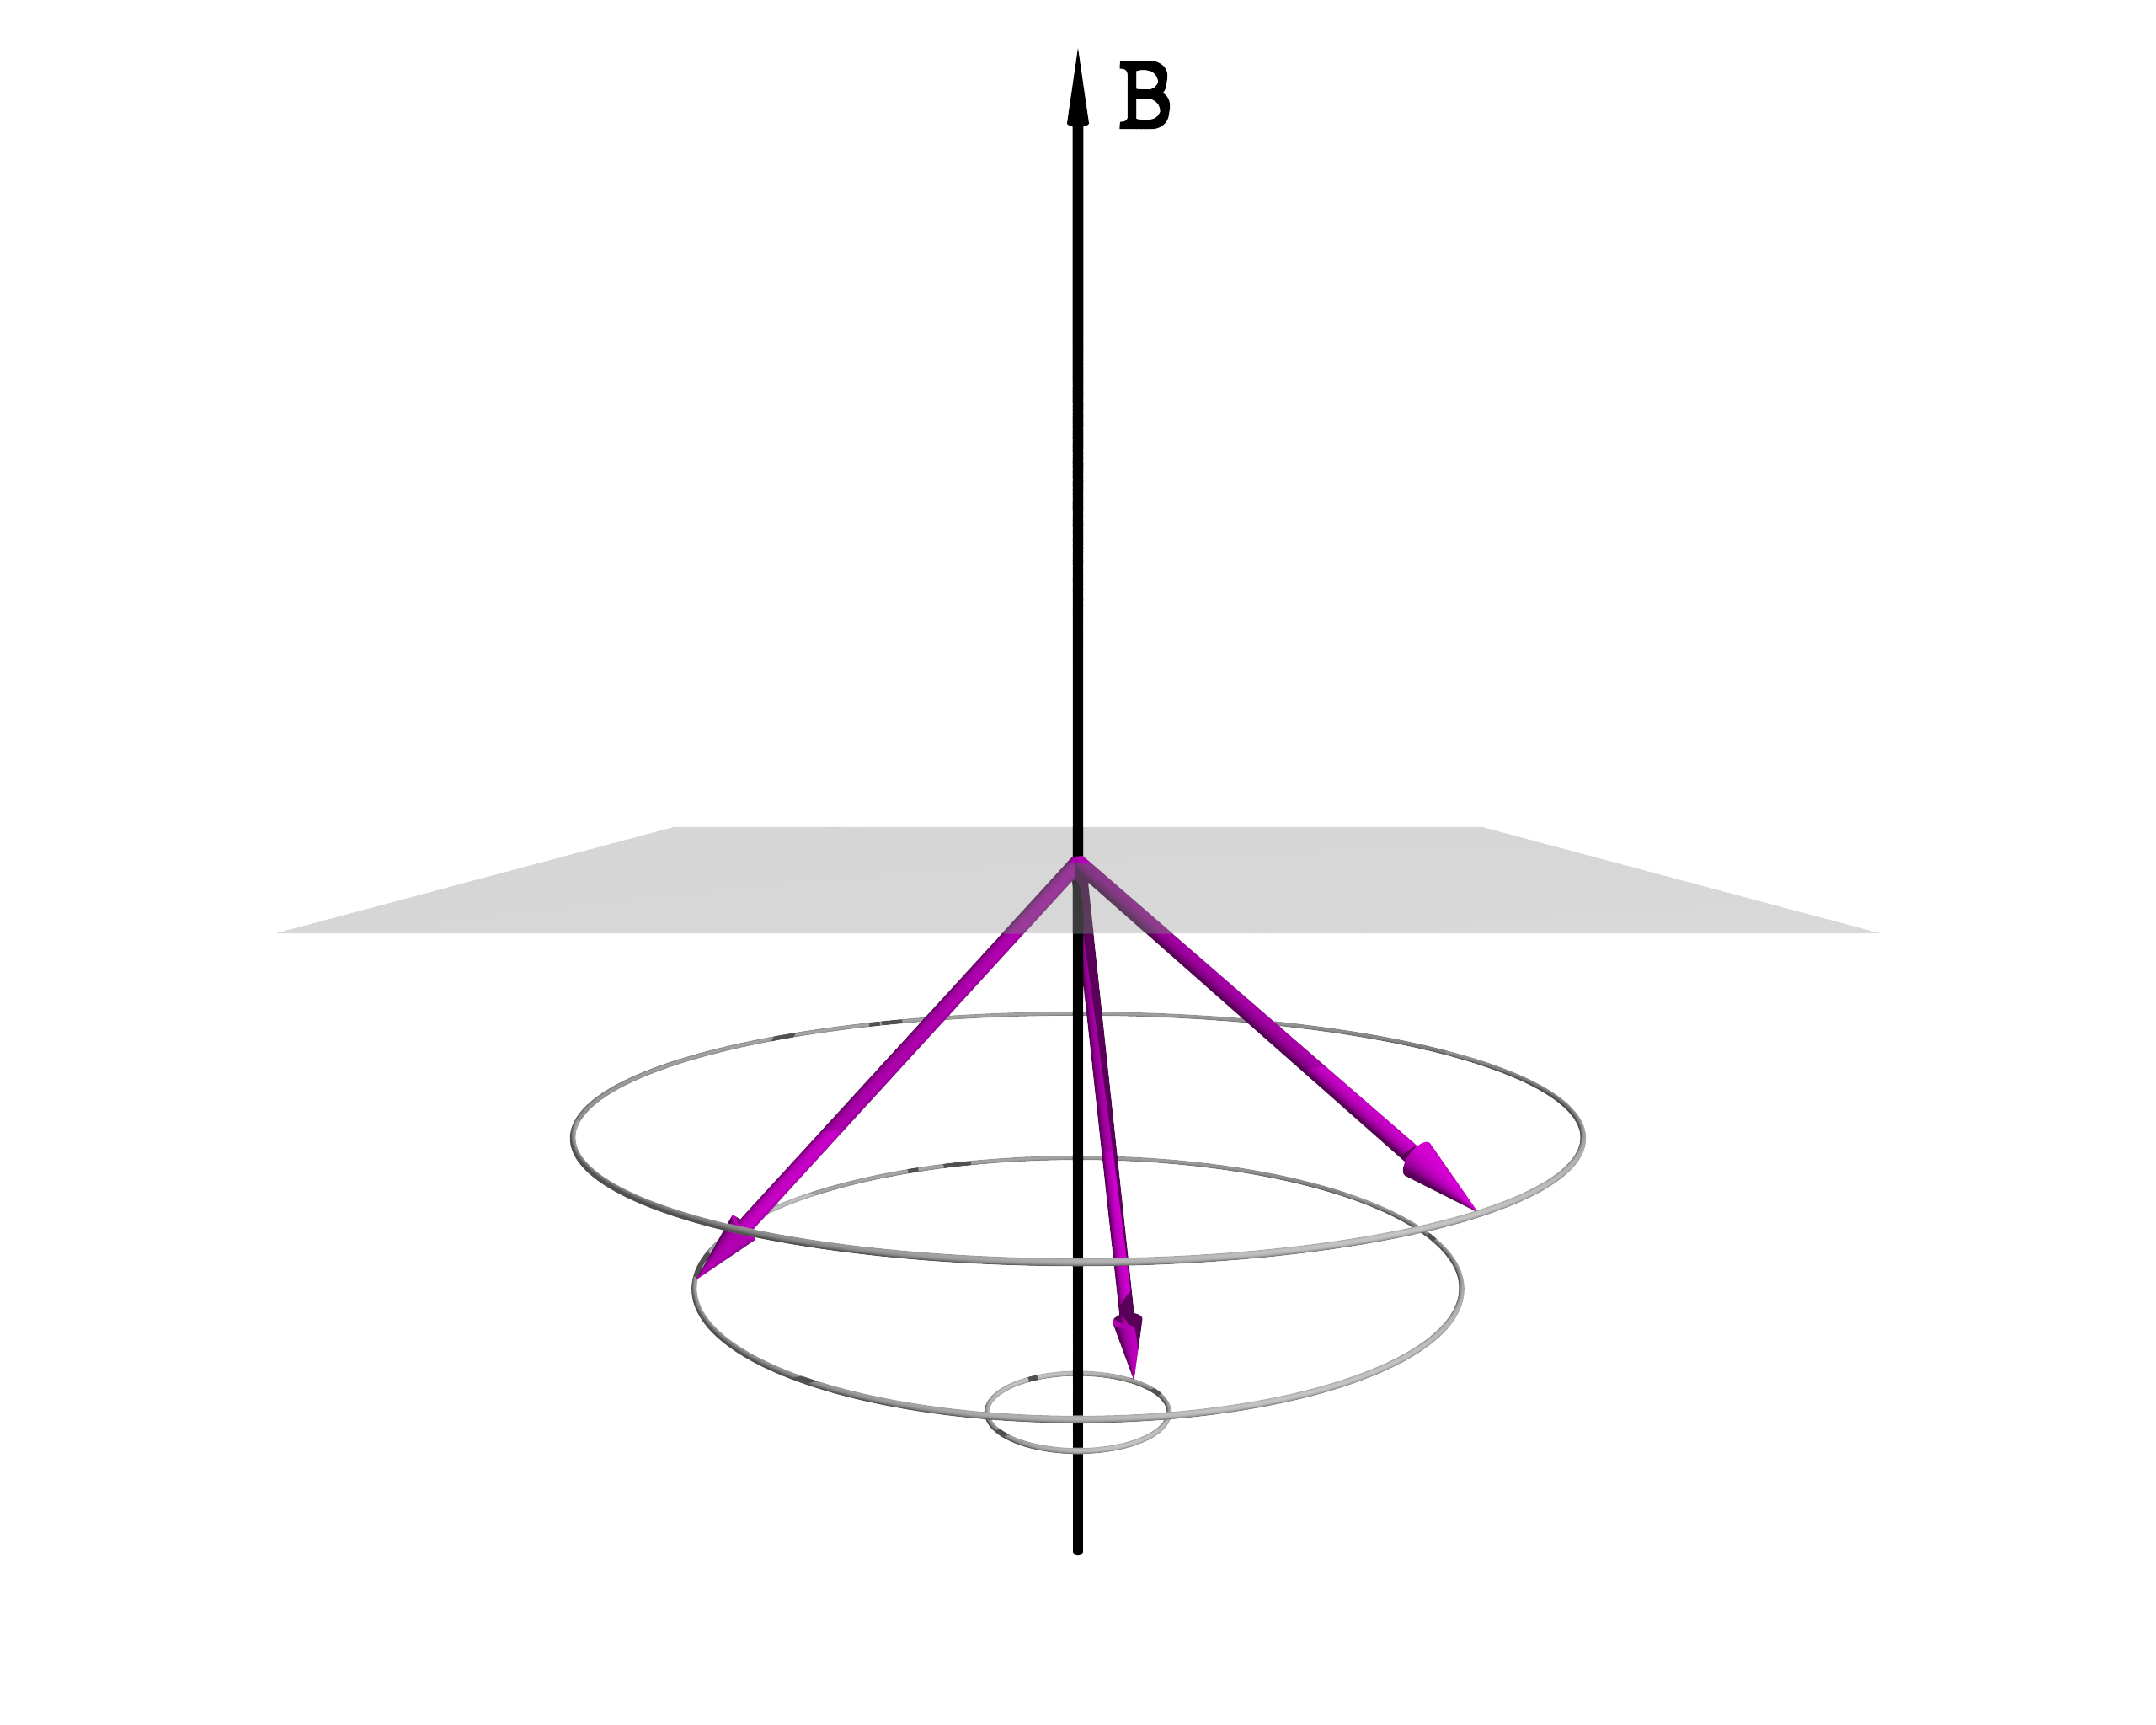
\includegraphics[height=5.5cm]{./mri/pic/Spin2}
		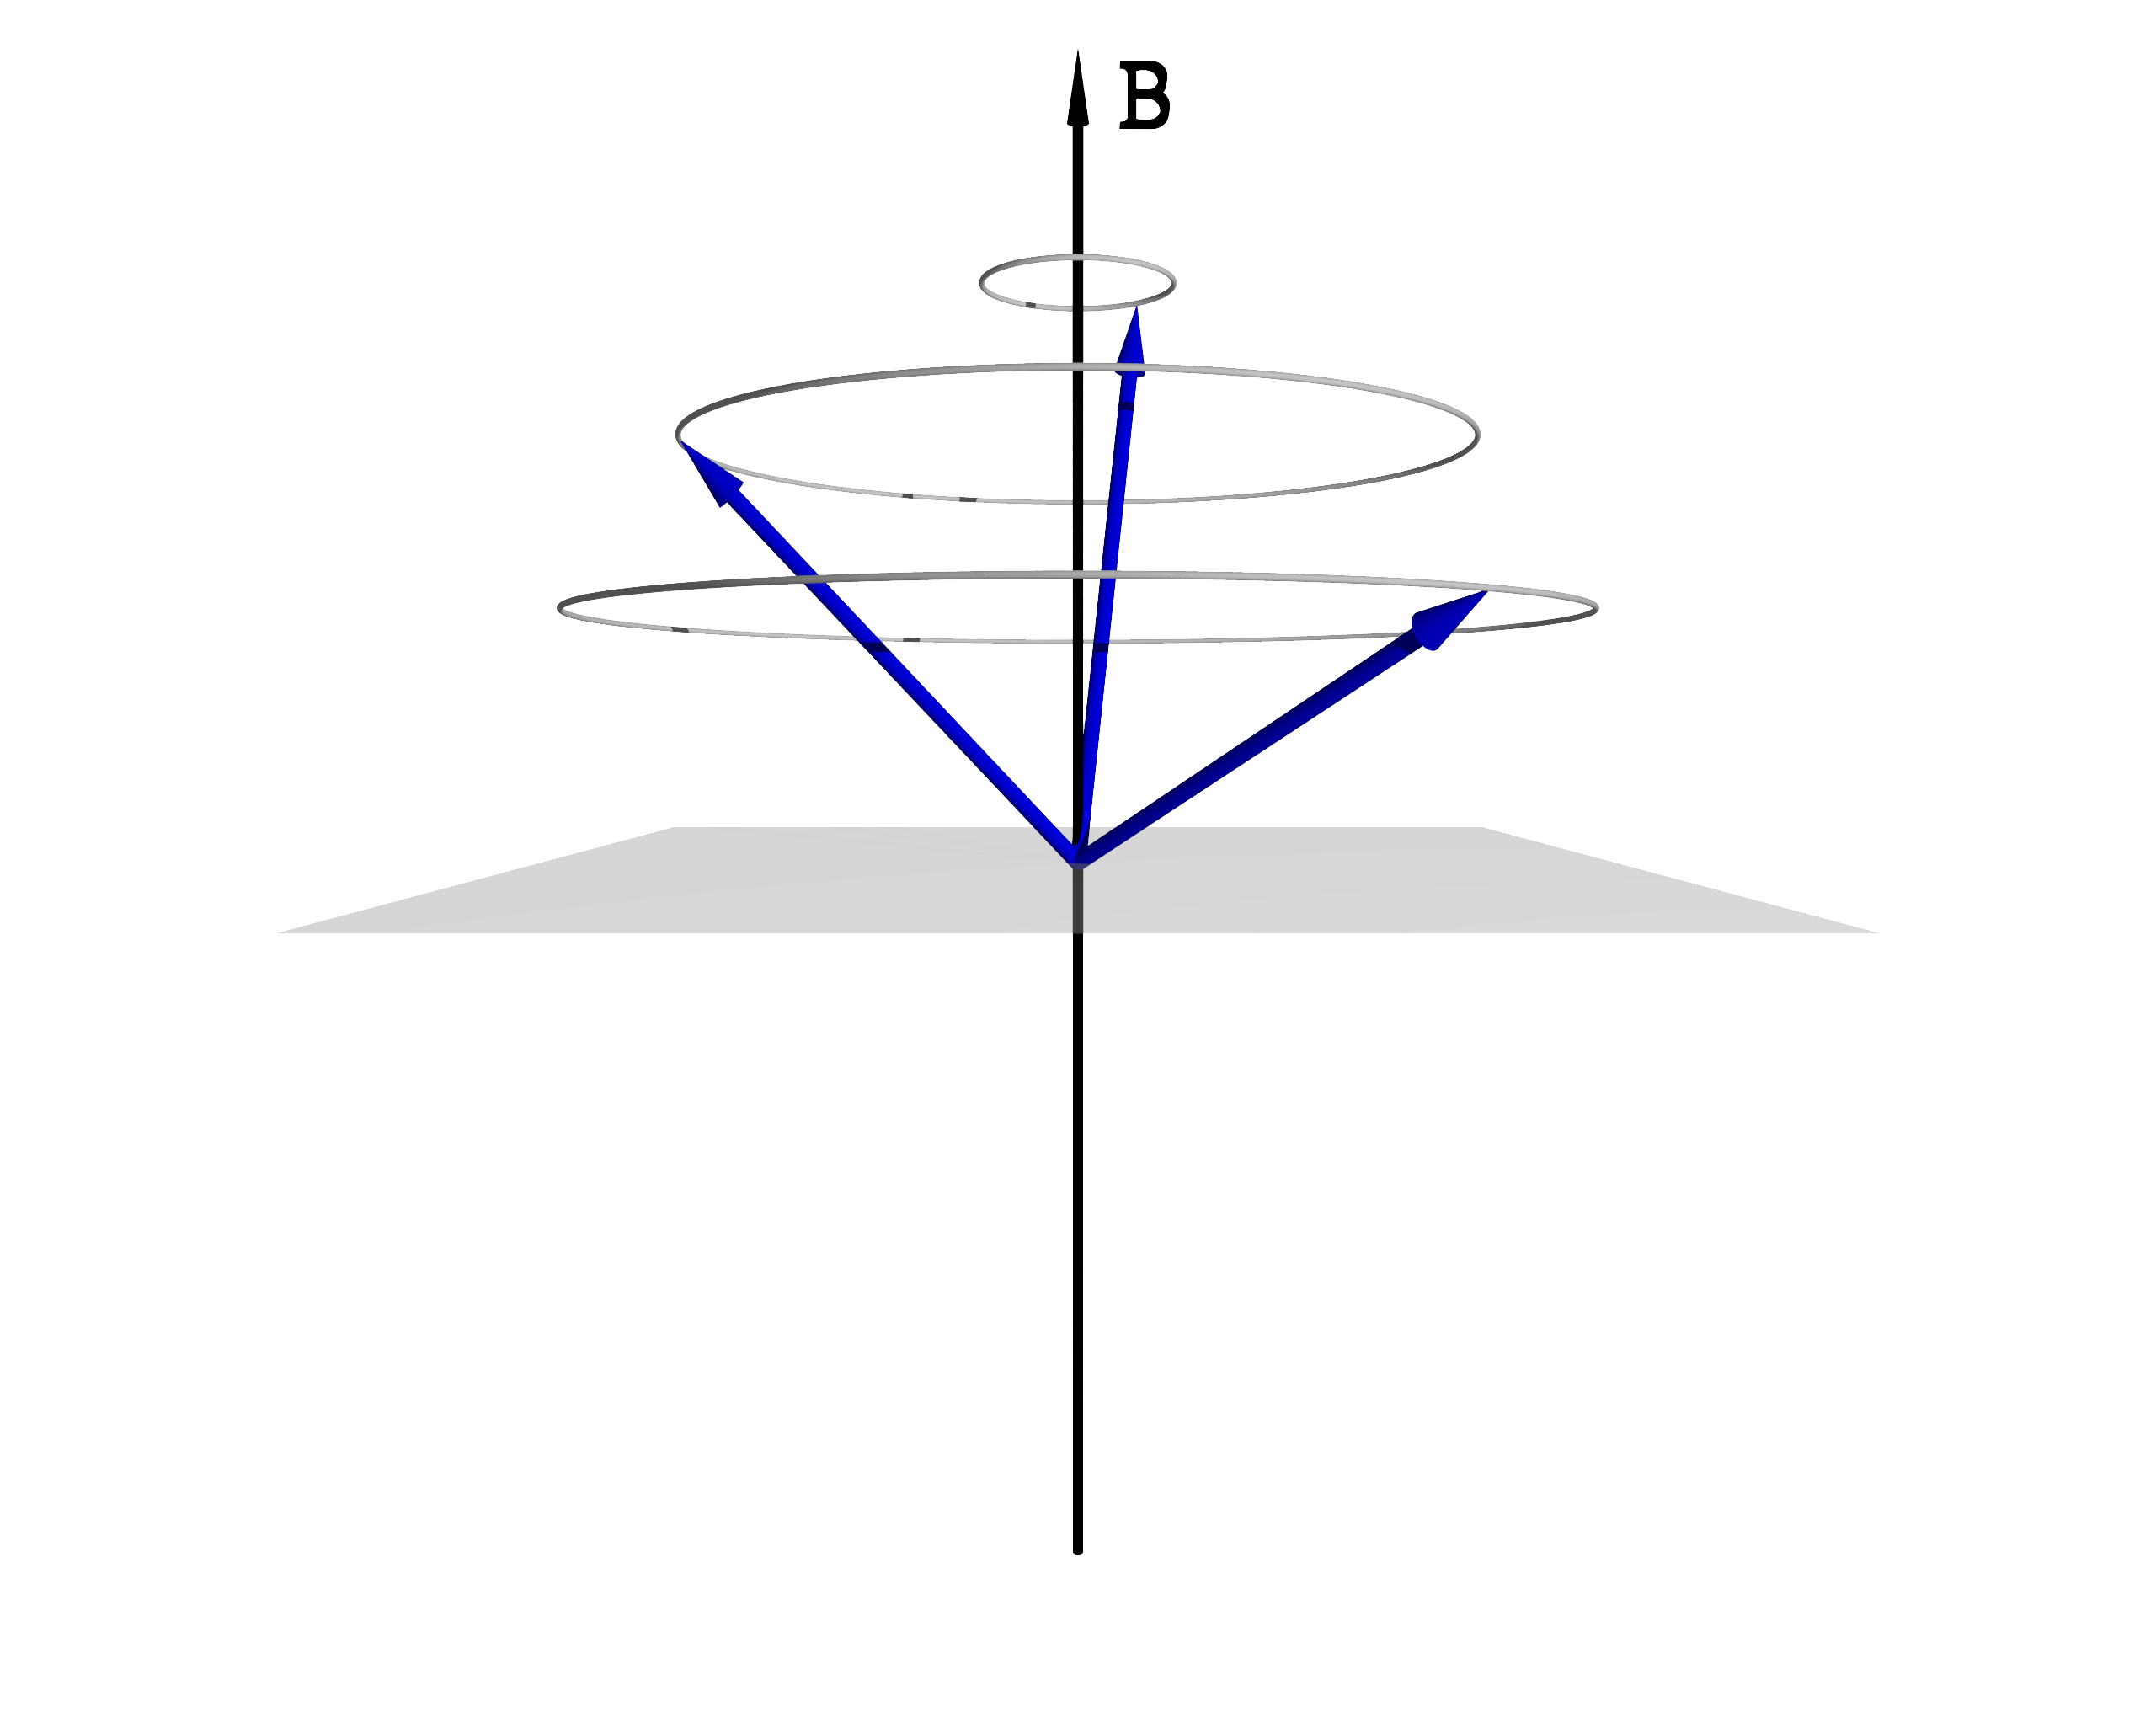
\includegraphics[height=5.5cm]{./mri/pic/Spin1}
		\caption{Links, der energetisch niedrigere Zustand und rechts der h"ohere Zustand. Dabei k"onnen die Winkel $\theta$ innerhalb der Zust"ande alle beliebigen Werte annehmen.}
		\label{fig:spin}
	\end{figure}
	
	Wie in n"achsten Kapitel genauer beschrieben wird, k"onnen zwei Zust"ande identifiziert werden, die klassisch den Situationen in Abbildung \ref{fig:spin} entsprechen. Sie unterscheiden sich durch das Vorzeichen von $-\vec{\mu} \cdot\vec{B}$. Im quantenmechanischen Modell werden dies zwei klar unterscheidbare Zust"ande mit unterschiedlichen Energien sein.
	
	\subsection{Hochfrequenzimpuls}
	
	Damit die Protonendichte gemessen werden kann, m"ussen die Protonen zum Strahlen angeregt werden. Dies ist mit einem Hochfrequenzimpuls mit Larmorfrequenz m"oglich. Durch einen solchen Impuls werden zwei Effekte erzielt:
	

	
	\begin{enumerate}
		\item Alle Protonen pr"azedieren in Phase. Bildlich kann man sich das Hochfrequenzfeld als ein sich rotierenden Magneten vorstellen. Diese Rotation bringt alle Dipolmomente der Protonen in Phase.
		\item Alle Protonen werden in den gleichen, energetisch h"oheren Zustand gebracht (Abbildung \ref{fig:spin} rechts).
	\end{enumerate}
	
	Dadurch, dass die Protonen in Phase pr"azidieren, erzeugen sie ein messbares Magnetfeld $\vec{M}_{XY}$ senkrecht zum Magnetfeld $\vec{B}_0$. Jedes dieser Protonen hat auch vorher schon ein Magnetfeld $\vec{M}_i$ erzeugt, welche jedoch wegen der destruktiver Interferenz nicht messbar waren.
	
	Weil sich nun alle Protonen im gleichen Zustand befinden, ist ein weiteres Magnetfeld $\vec{M}_{Z}$, das die selbe Ausrichtung wie das Magnetfeld $\vec{B}_0$ hat, messbar. Auch diese Magnetfelder war bereits vorhanden, hat sich aber ebenfalls aufgehoben, weil die beiden Zust"ande gleich stark waren.
	
	Kurz nach dem Impuls wollen die Protonen jedoch wieder in ihren Ausgangszustand zur"uck. Die Zeit die sie dazu ben"otigen wird durch die Zeitkonstante $T_1$ beschrieben.
	
	Aufgrund von kleinen Unregelm"assigkeiten im Magnetfeld, geraten die Protonen ausser Phase. Dieser Prozess ist langsamer als der Vorherige und wird mit der Zeitkonstante $T_2$ beschrieben.
	
	\subsection{Messgeometrie}

	\begin{figure}
		\centering
		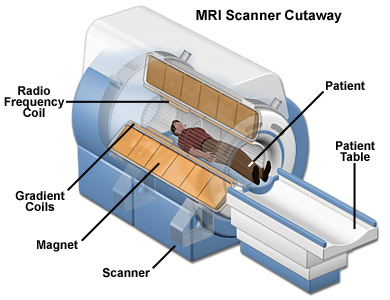
\includegraphics[width=0.48\hsize]{./mri/pic/mri_scanner.jpg} 
		\quad
		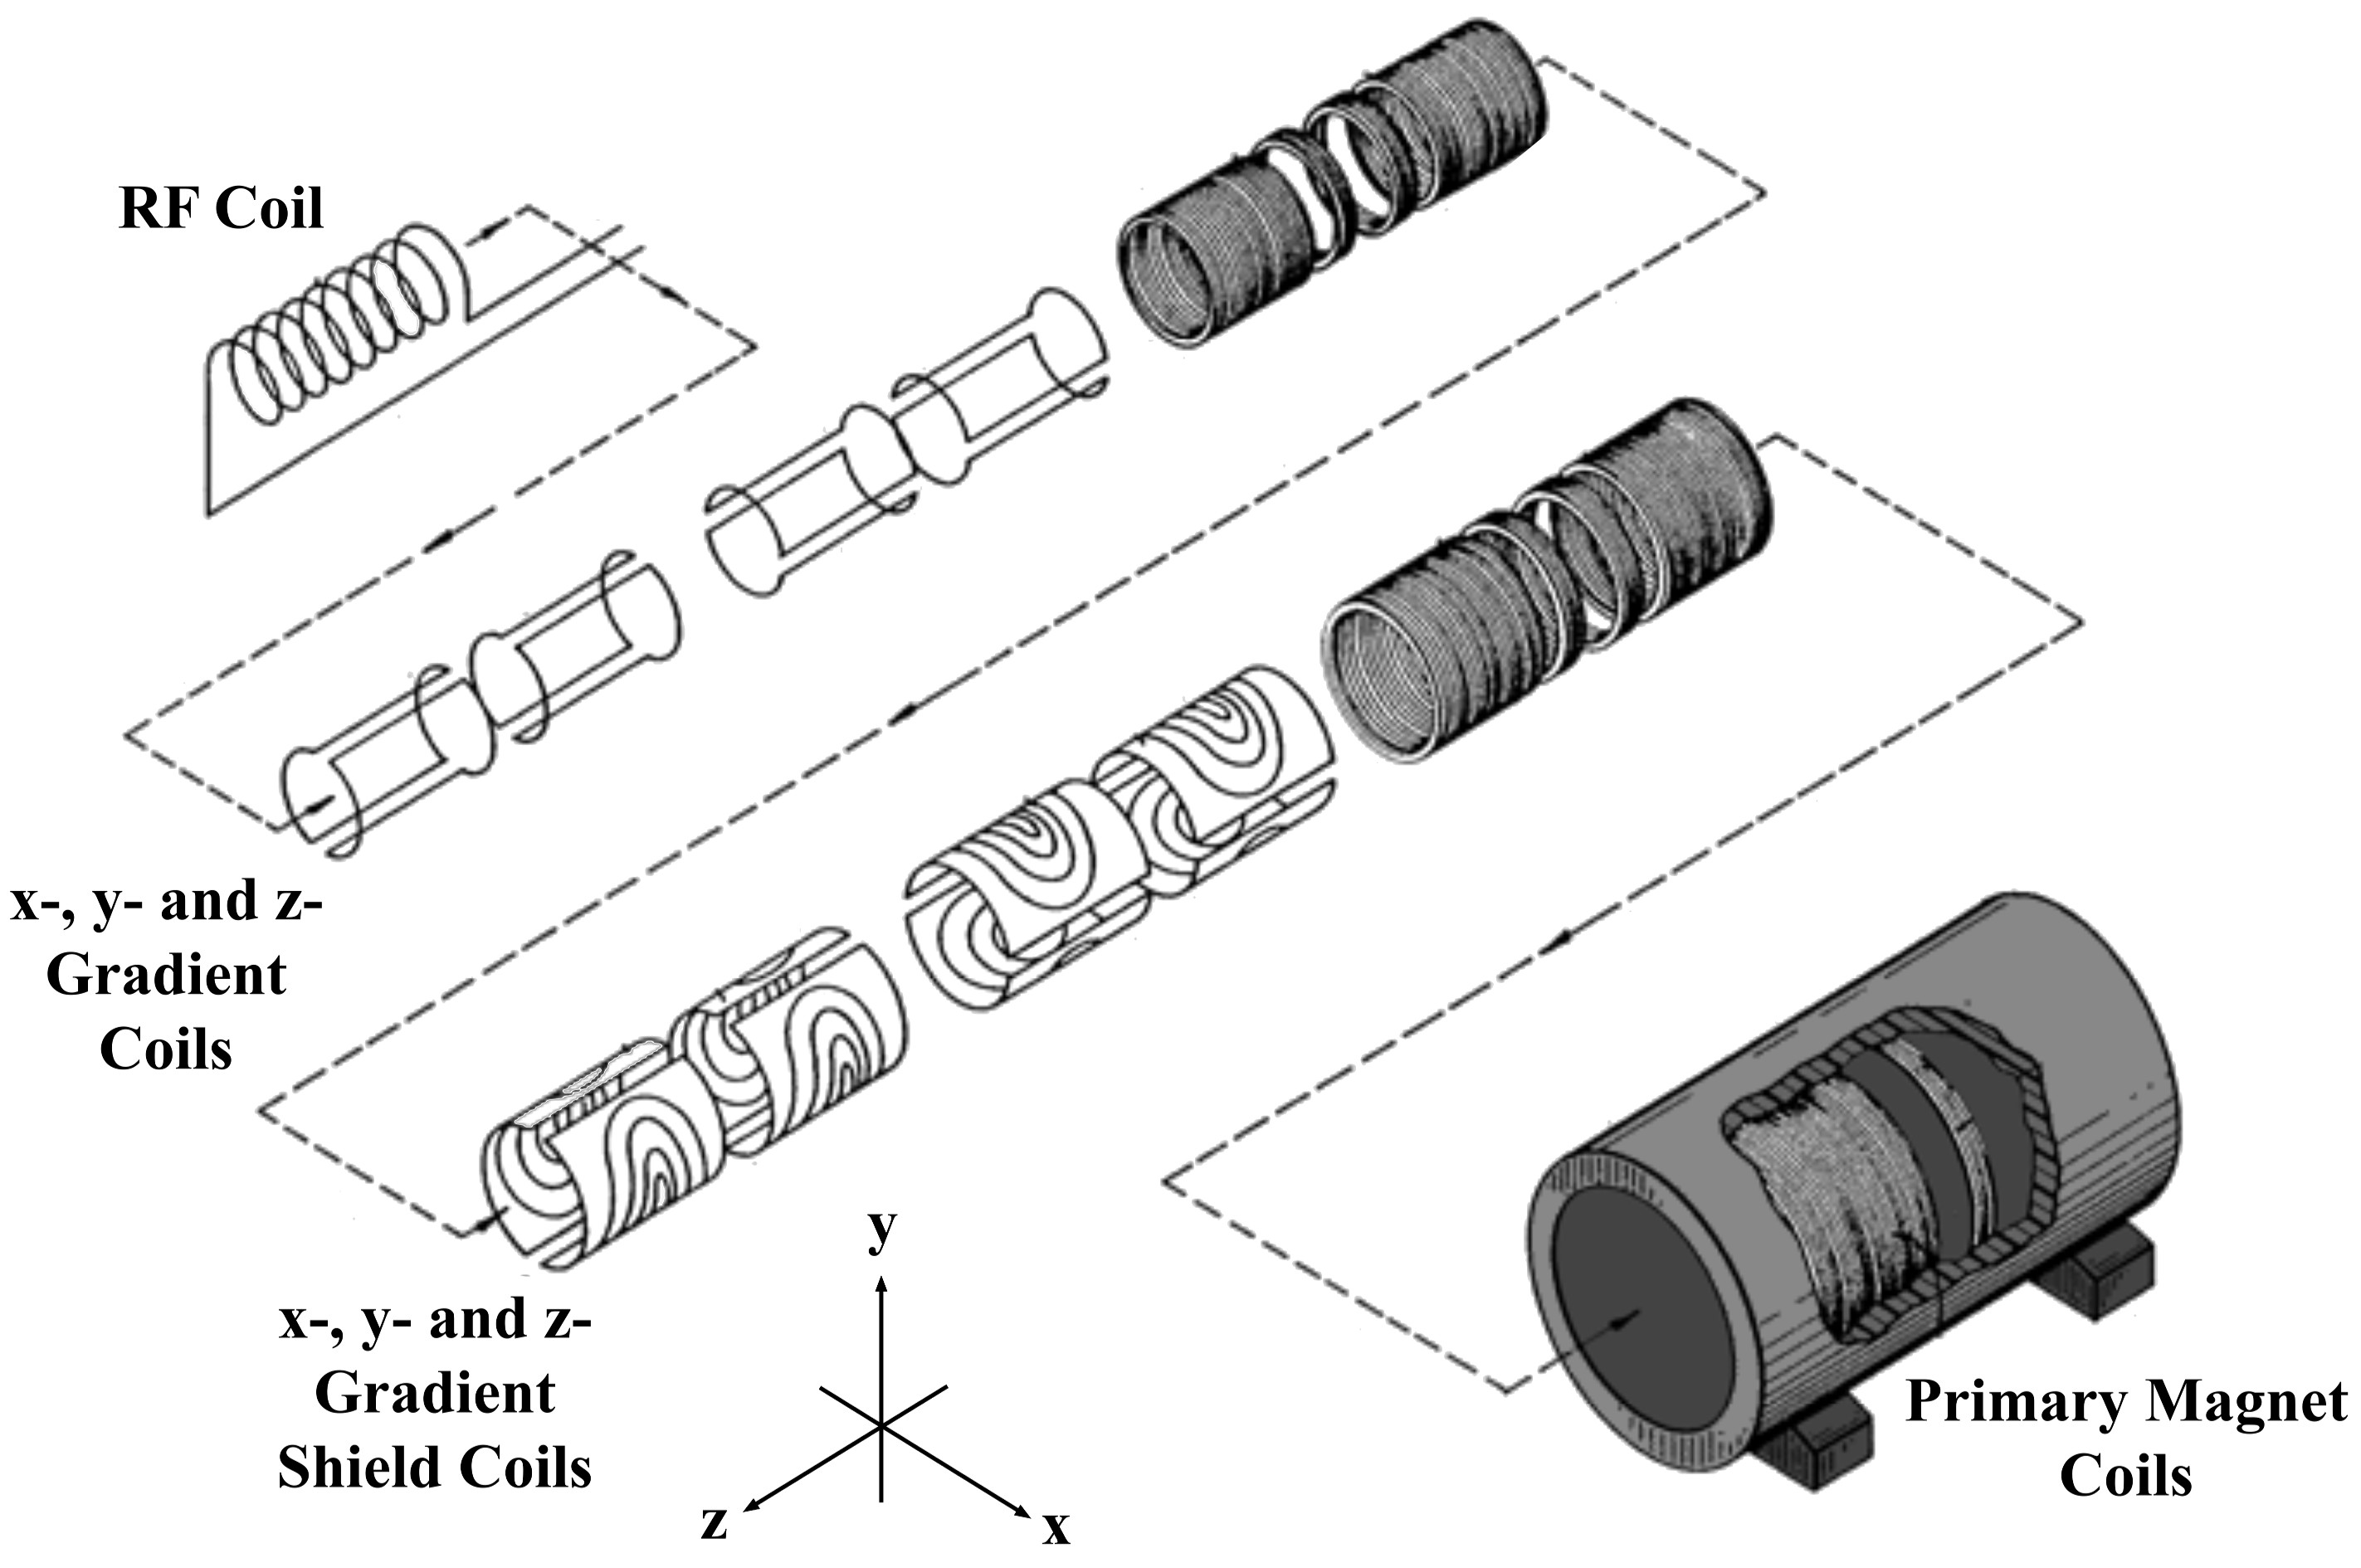
\includegraphics[width=0.48\hsize]{./mri/pic/gradientfield.jpg}
		\caption{Links die Hauptbestandteile eines MRI-Scanners und rechts die Zusammensetzung der verschiedenen Spulen \cite{MRIScanner}\cite{gradients}.}
		\label{fig:MRIScanner}
	\end{figure}

	Ziel ist es, anhand verschiedenen Messungen der Protonendichte aus verschiedenen Winkeln und Abst"anden, ein Bild zu erzeugen. Dazu wird ein inhomogenes Magnetfeld benutzt, dessen St"arke in eine Richtung zunimmt. Mit der richtigen magnetischen Flussdichte und der dazugeh"origen Frequenz werden die Protonen angeregt. 
	
	Mit Hilfe von Gradientenspulen (Abbildung \ref{fig:MRIScanner} links) wird ein Magnetfeld erzeugt, das in einer Ebene konstant ist. Der anschliessende Hochfrequenzimpuls regt die Protonen dieser Ebene an. Dazu wird eine schmalbandige Spule ben"otigt, in Abbildung \ref{fig:MRIScanner} links, als RF-Spule (engl. \emph{Radio Frequency}) angeschrieben. Die Protonen emittieren kurz nach der Anregung Strahlung, die mit der selben Spule gemessen werden kann.
	
	Aus den verschiedenen Ebenen, die vom Winkel und von der Position abh"angig sind, kann mit der Radon-Transformation \cite{Mathsem} ein Bild berechnet werden.
	

%\section{Grundlagen}
%
%In diesem Abschnitt soll das Prinzip des MRI mit Hilfe der klassischen Physik erkl"art werden. Auf die quantenmechanischen Eigenschaften wird in Abschnitt \ref{sec:quant} eingegangen. Um das MRI Verfahren besser beschreiben zu k"onnen, wird das Modell eines Protons benutzt.
%
%\subsection{Magnetismus}
%
%%TODO
%%Um das MRI Verfahren zu verstehen ist es wichtig, dass der Magnetismus verstanden wurde. An dieser Stelle werden noch einmal die wichtigsten Eigenschaften erl"autert.
%Um das MRI Verfahren zu verstehen ist es wichtig, dass die Grundlagen des Magnetismus verstanden wurden. An dieser Stelle werden noch einmal die wichtigsten Eigenschaften erl"autert.

%verschiedene Magnetfeldst�rken, bis 0.5 Tesla Permanentmagnete
%
%\section{Grundlagen}
%
%\subsection{Magnetismus}
%
%\subsection{Pr�zession}
%
%\begin{figure}
%	\centering
%	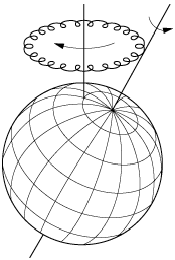
\includegraphics[height=4cm]{./mri/pic/praezession}
%	\caption{Pr�zession \cite{praezession}}
%	\label{fig:spin}
%\end{figure}
%
%\subsubsection{Larmor-Pr�zession}
%
%
%
%\subsection{NMR -- Nuclear Magnetic Resonance}
%
%\subsection{MRI Signal}


%Jeder Magnet erzeugt in sich geschlossene Feldlinien. Sie f"uhren vom magnetischen Nordpol zum magnetischen S"udpol. Auch jeder mit elektrischem Strom durchgeflossene Leiter erzeugt ein magnetisches Feld (Abbildung \ref{fig:magnetismus}). Dabei wird die elektrische Feldst"arke $H$ oder die magnetische Flussdichte $B$ angegeben \cite{wiki:magnetismus}.
%
%\begin{figure}
%	\centering
%	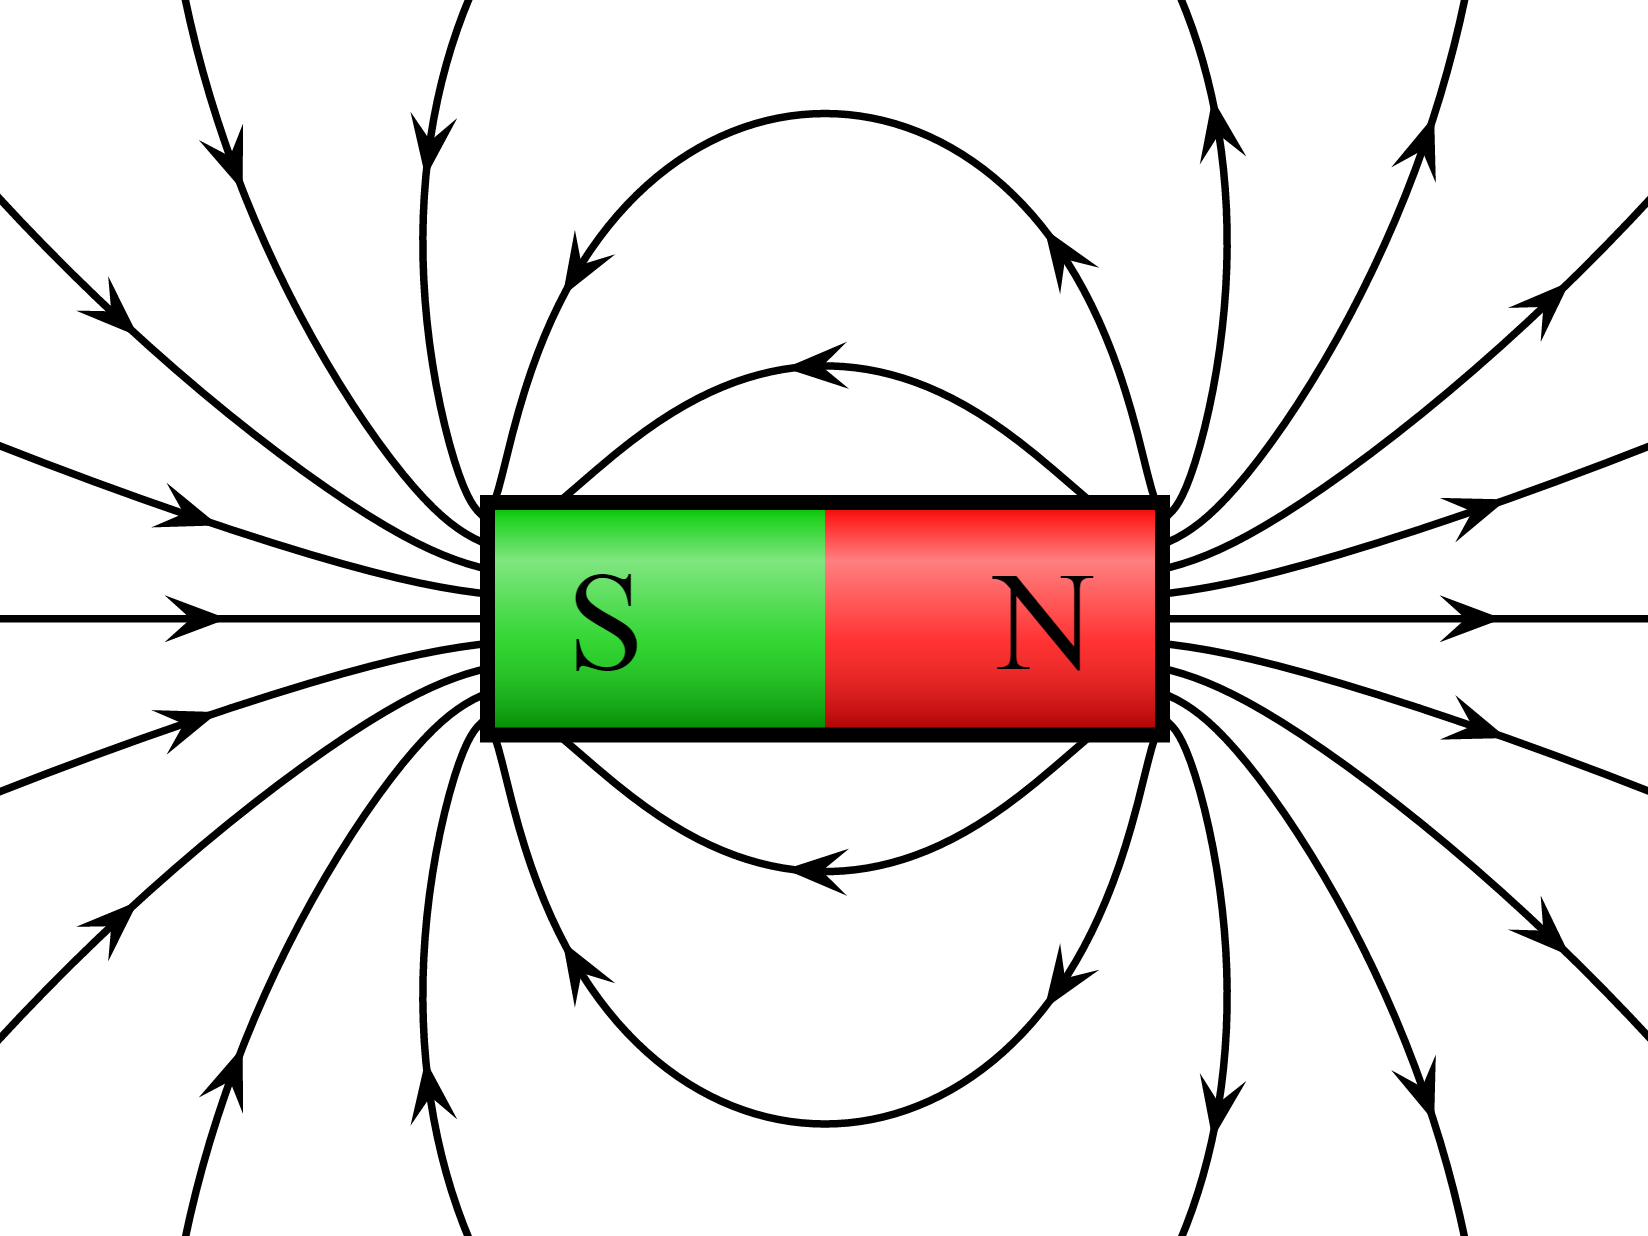
\includegraphics[height=2.5cm]{./mri/pic/mag1}
%	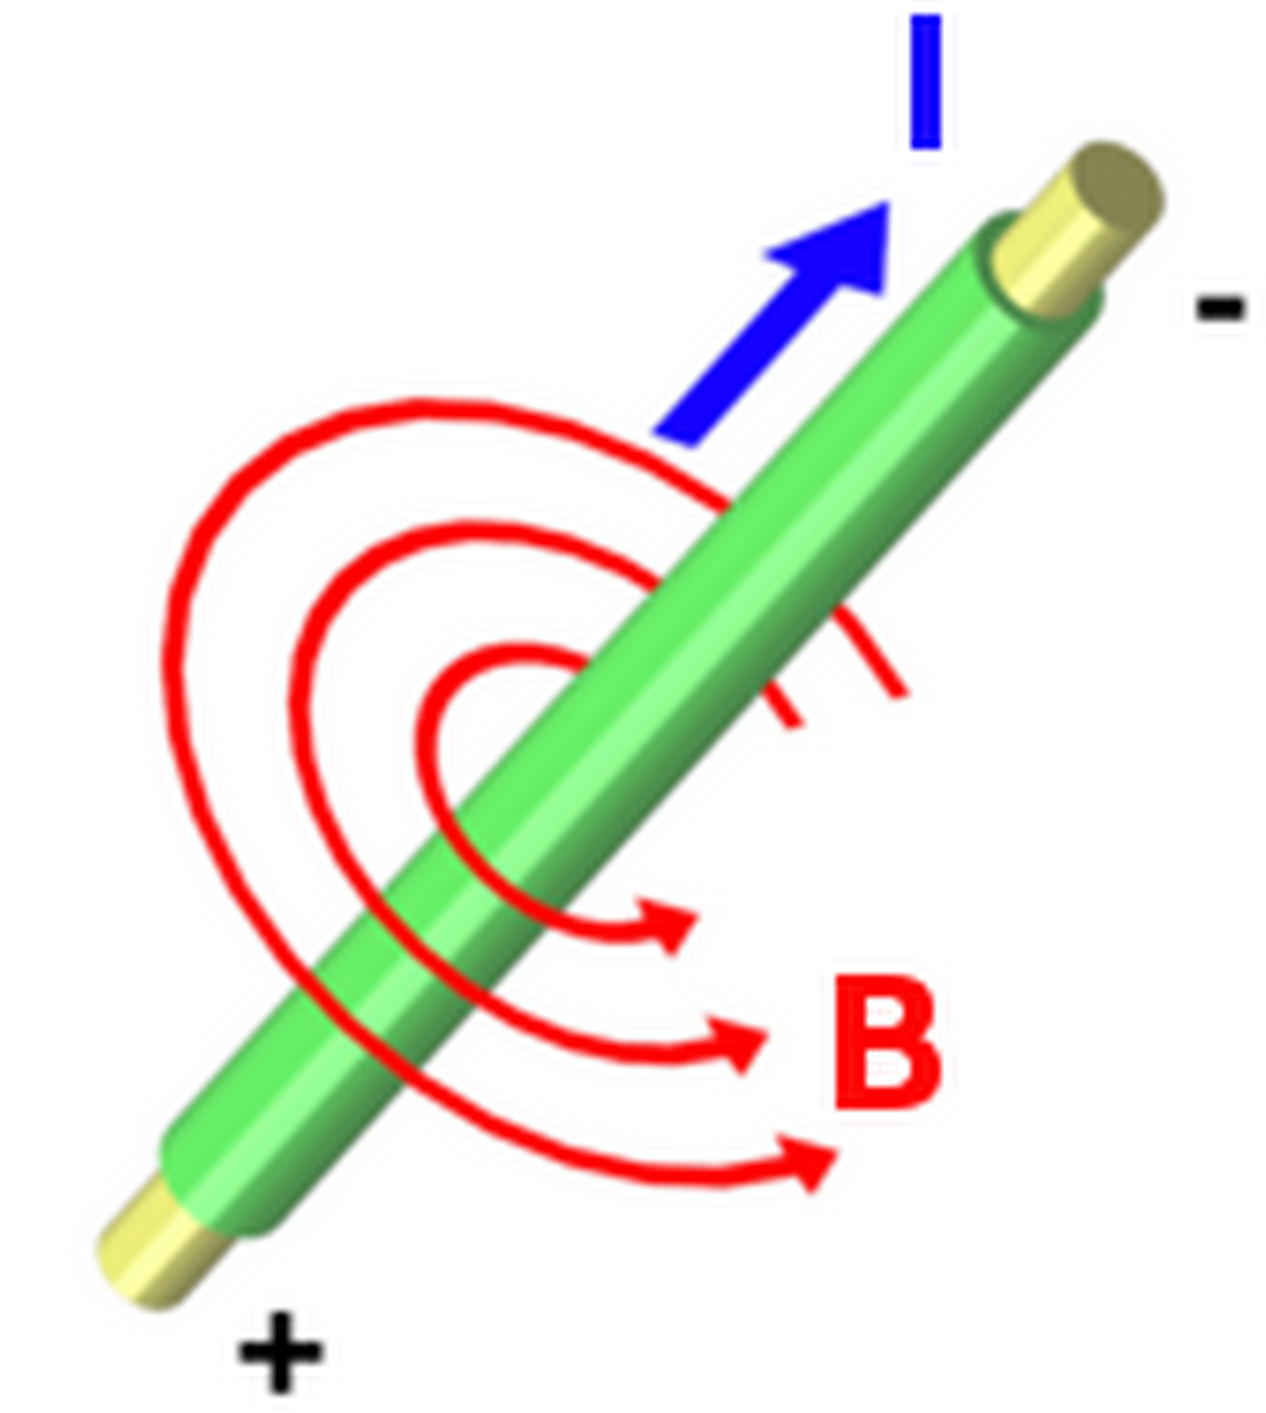
\includegraphics[height=2.5cm]{./mri/pic/mag2}
%	\caption{Magnetismus: Links ein Stabmagnet, der mit in sich geschlossenen Feldlinien umgeben ist. Rechts ein Leiter der mit elektrischem Strom durchflossen ist. \cite{wiki:magnetismus}}
%	\label{fig:magnetismus}
%\end{figure}

%\subsection{Pr"azession}
%
%Ein einfaches Modell eines Protons ist ein Stabmagnet. Der Nord- und der S"udpol dieses Magneten liegen nicht perfekt auf einer Linie mit der Rotationsachse des Protons. Die Rotationsachse taumelt, was als Pr"azession bekannt ist (Abbildung \ref{fig:praezession}). Eine Analogie da zu ist ein Kreisel, der immer langsamer wird und beginnt zu taumeln. 
%Die Frequenz, mit der sich das Proton um die Achse des Magnetfeld dreht, ist $\omega_p$. Sie ist nicht mit der Frequenz der Drehung des Protons selber zu verwechseln.
%
%\begin{figure}
%	\centering
%	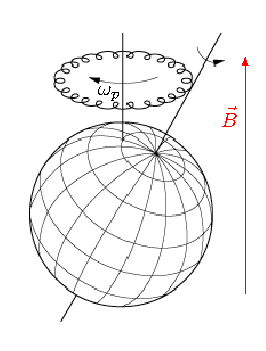
\includegraphics[height=5cm]{./mri/tikz/precession}
%	\caption{Pr"azession: Modell eines Protons das sich in einem Magnetfeld $\vec{B}$ befindet,  \cite{praezession}}
%	\label{fig:praezession}
%\end{figure}
%
%
%
%\subsection{NMR -- Nuclear Magnetic Resonance }\label{mri:grundlagen:NMR}
%
%\begin{figure}
%	\centering
%	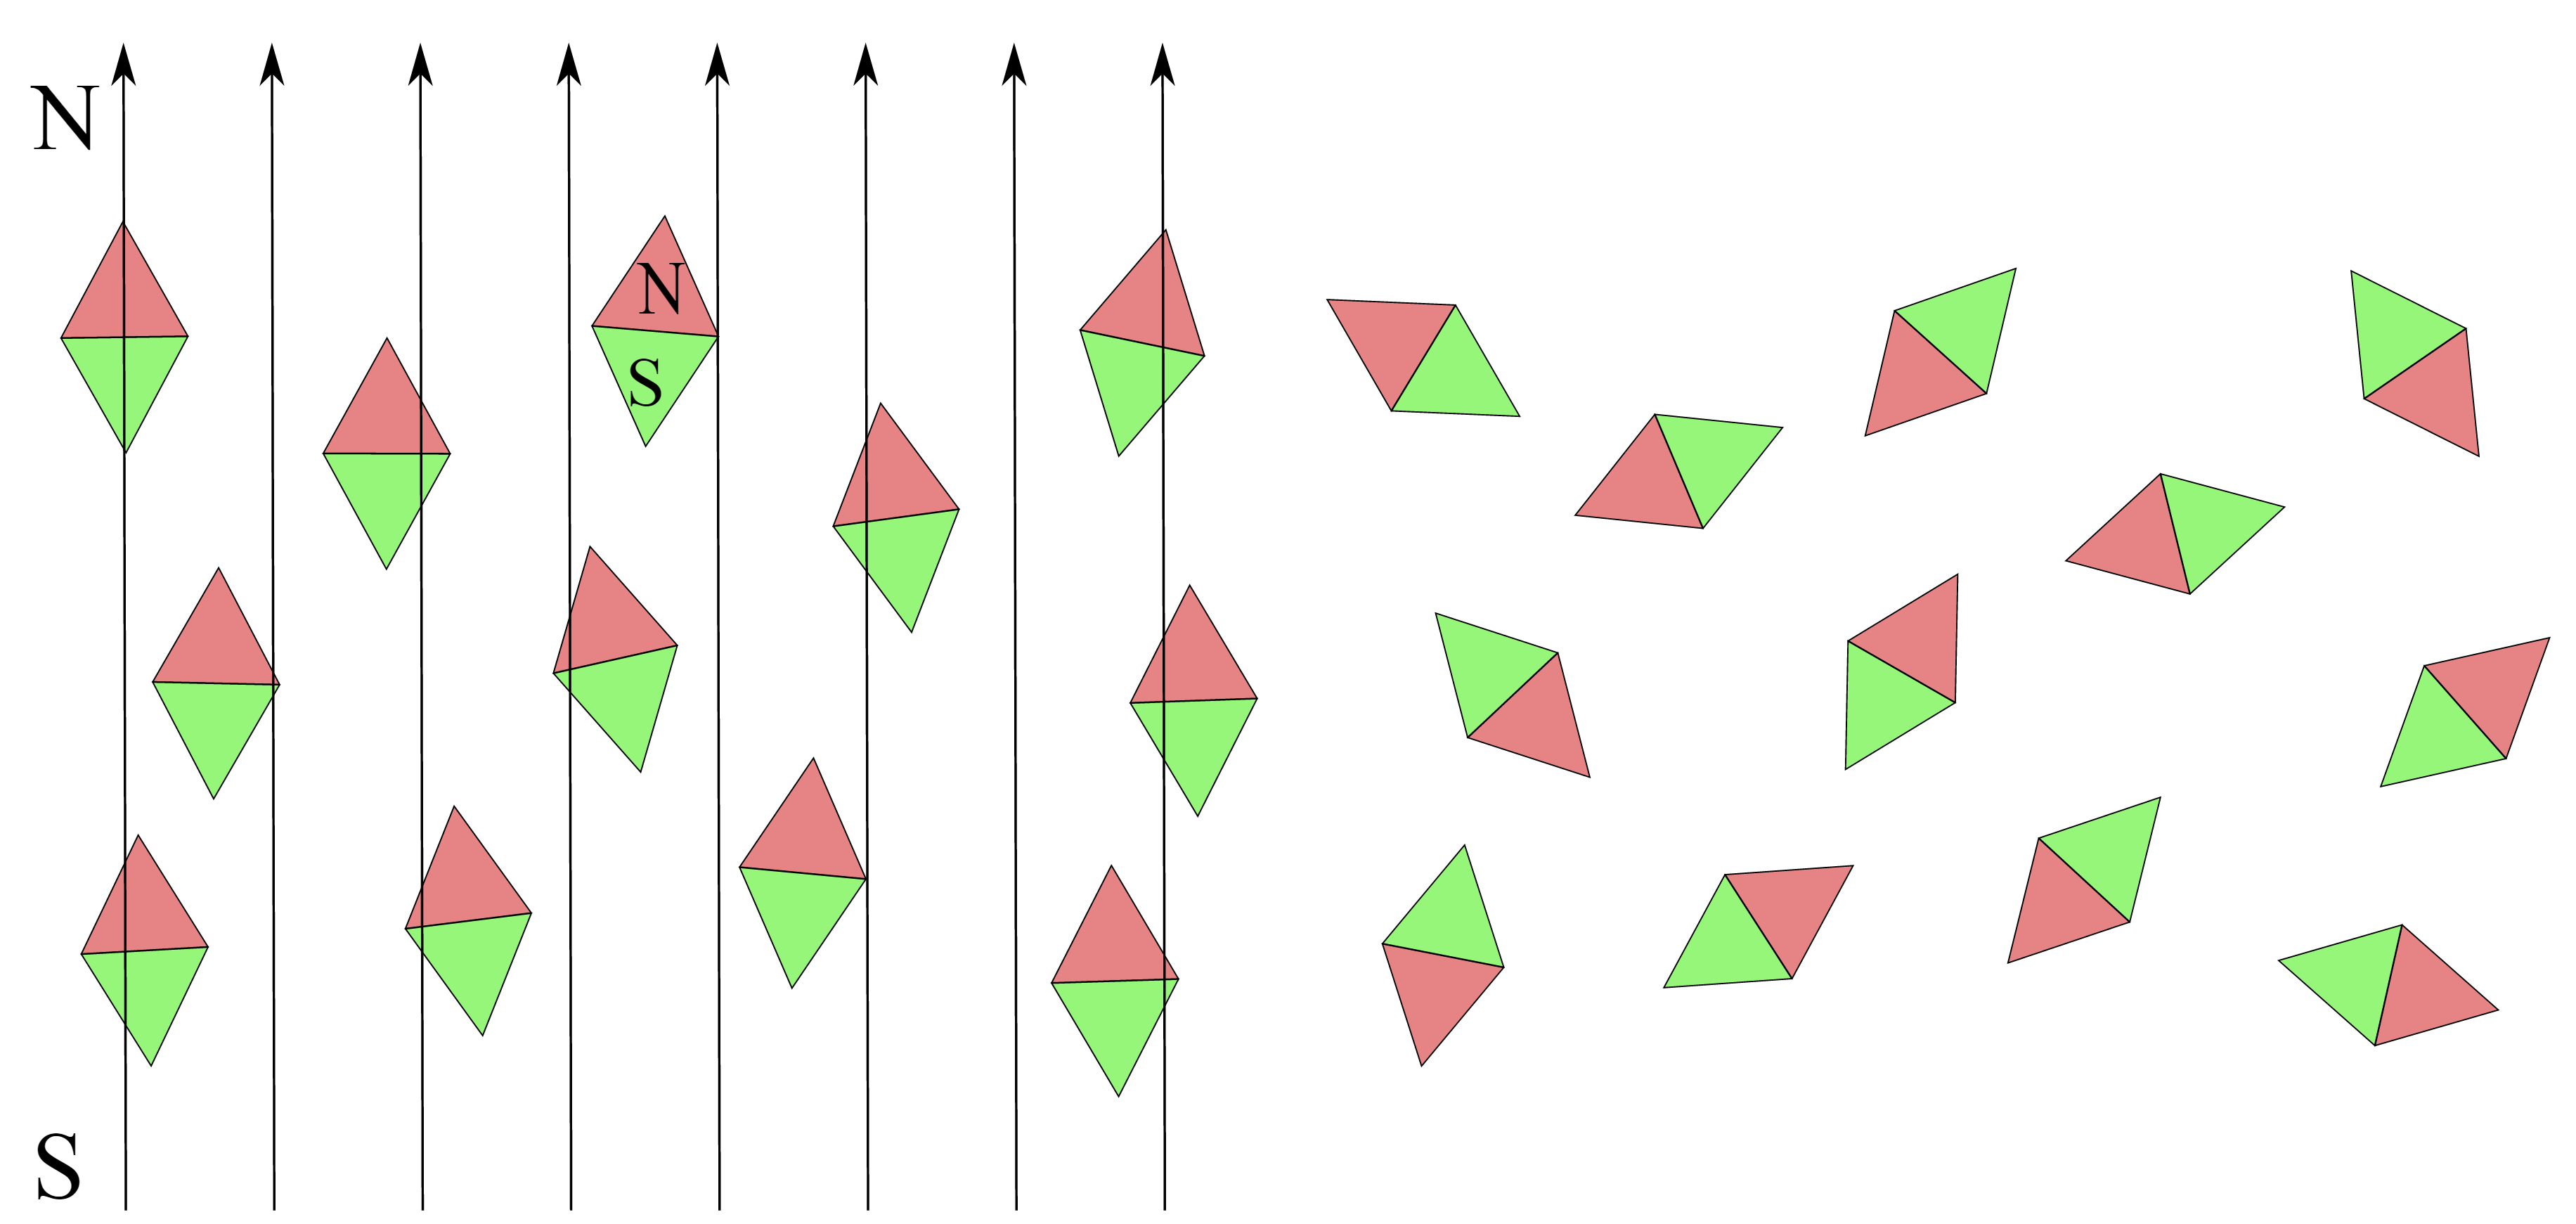
\includegraphics[height=4cm]{./mri/pic/mag3}
%	\caption{Links: Mehrere Protonen, als Stabmagnete gezeichnet, richten sich dem Magnetfeld aus. Rechts: Protonen im Ausgangszustand \cite{wiki:magnetismus}}
%	\label{fig:magnetismus2}
%\end{figure}
%
%Wenn nun mehrere solche Protonen mit einem statischen Magnetfeld angeregt werden, richten sich diese aus. Dabei gibt es zwei Zust"ande: Den stabilen Zustand, indem sich die Protonen parallel zum Magnetfeld ausrichten. Dabei ist die Polarisierung des externen Magnetfelds und die des Protons N--S--N--S. Im zweiten, instabilen Zustand, ist die Ausrichtung N--N--S--S und damit energetisch h"oher, die Protonen richten sich anti-parallel aus, also um 180$^{\circ}$ gedreht (Abbildung \ref{fig:magnetismus2} links). 
%
%Die Protonen k"onnen vom niedrigeren Zustand in den h"oheren Zustand wechseln in dem sie ein Photon absorbieren. Wenn sie den Zustand erneut wechseln, geben sie ein Photon ab. Die Energie $E$ des Photons muss dabei exakt stimmen, damit ein Wechsel m"oglich ist. Die Energie des Photons ist von dessen Frequenz $f$ und von der Planck'schen Konstanten $h$ abh"angig \cite{MRI:Joseph}.
%\begin{equation}
%E= h\cdot f
%\end{equation}
%Die Frequenz entspricht der Larmorfrequenz $f = f_{Larmor}$
%
%\subsubsection{Bolzmannstatistik}
%
%Wenn sich nun mehrere Protonen in einem Magnetfeld befinden, richtet sich ein Teil parallel, im niedrigieren Zustand $N^{+}$, aus und ein Teil richtet sich anti-parallel, im h"oheren Zustand $N^{-}$, aus. Die Verteilung ist temperaturabh"angig
%\begin{equation}
%\dfrac{N^{-}}{N^{+}}= e^{-E/kT}
%\end{equation}
%$E$ ist die Energiedifferenz zwischen den Spinzust"anden, $k$ ist die Bolzmannkonstate und $ T$ ist die Temperatur in Kelvin.
%
%Jedes Proton erzeugt sein eigenes kleines Magnetfeld $\vec{M}_{Z,i}$, das in der $Z$-Achse liegt. Die Summe all dieser Vektoren ist proportional zu $N^{+}-N^{-}$.
%\begin{equation}
%\displaystyle \sum_{i} \vec{M}_{Z,i} =\vec{M}_Z
%\end{equation}   
%
%\subsubsection{$T_1$ Prozess}
%
%Im Gleichgewicht liegt die Gesamtmagnetisierung $\vec{M}_Z$, auch Longitudinal-Magnetisierung genannt, in Richtung des externen Magnetfeldes $\vec{B}_0$. Sie wird im folgenden $\vec{M}_0$ genannt. In dieser Ausgnagslage gibt es keine Transversal-Magnetisierungen $\vec{M}_X$ oder $\vec{M}_Y$.
%
%Wenn dem System nun genug Energie zugef"uhrt wird, ist es m"oglich, das System zu s"attigen, so dass $\vec{M}_Z=0$. Das System wird aber nach einer gewissen Zeit wieder im Ausgangszustand sein, dabei gibt es Energie, bzw. Photonen ab. Diese Zeit wird durch die Zeitkonstante $T_1$ beschrieben (engl. spin lattice relaxation time).
%\begin{equation}
%{M}_{Z}= M_0\left(1-e^{-t/T_1}\right)
%\end{equation}
%
%\subsubsection{$T_2$ Prozess}
%
%Kurz nachdem das System in den energetisch h"oheren Zustand gebracht wurde, haben alle Protonen die gleiche Pr"azessionsfrequenz und sind phasengleich ausgerichtet. Aufgrund von kleinen Unterschieden im Magnetfeld beginnen sie jedoch aus dem Takt zu geraten und rotieren mit ihrer eigenen Larmorfrequenz. Dabei nimmt die Transversal-Magnetisierung $M_{XY0}$ ab. Diese Zeit wird mit der Zeitkonstante $T_2$ beschrieben (engl. spin-spin relaxation time).
%
%\begin{equation}
%M_{XY}=M_{XY0}e^{-t/T_2}
%\end{equation}
%Es gilt $T_2 \le T_1$. Es treten beide Prozesse, $T_1$ und $T_2$, gleichzeitig auf.
%
%\subsection{RF-Signal}
%
%Eine Spule in Richtung der $X$-Achse wird mit Wechselstrom angeregt (Abbildung \ref{fig:MRIScanner}). Sie erzeugt dabei ein wechselndes Magnetfeld in Richtung der $X$-Achse. Man kann sich das vorstellen, als w"urde sich ein Magnet in der $XY$-Ebene um die $Z$-Achse rotieren. Wenn nun die Frequenz der Rotation mit der Larmorfrequenz "ubereinstimmt, bewegt sich das Magnetfeld der Spule relativ zu dem Protonen nicht.
%
%\subsubsection{MRI Signal}
%
%Wenn nun das alternierende Magnetfeld kurz eingeschaltet und dann wieder ausgeschaltet wird, kann die Relaxation gemessen werden. Dabei kann eine Spule als Sender und Empf"anger genutzt werden, weil das Empfangssignal die gleiche Frequenz wie das Sendesignal hat. Dieser gesendete Impuls ist k"urzer als $T_2$. Weil sich diese Frequenzen dieser Signales im Hochfrequenzbereich befinden werden sie als RF-Signale bezeichnet (engl. RF: Radio Frequency).
%
%\subsection{Das statische Magnetfeld}
%
%\begin{figure}
%	\centering
%	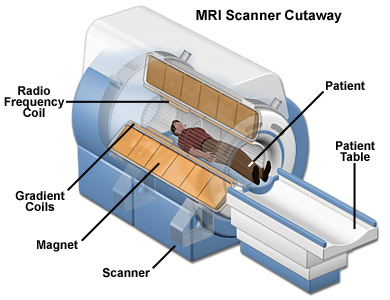
\includegraphics[width = 6cm]{./mri/pic/mri_scanner.jpg} 
%	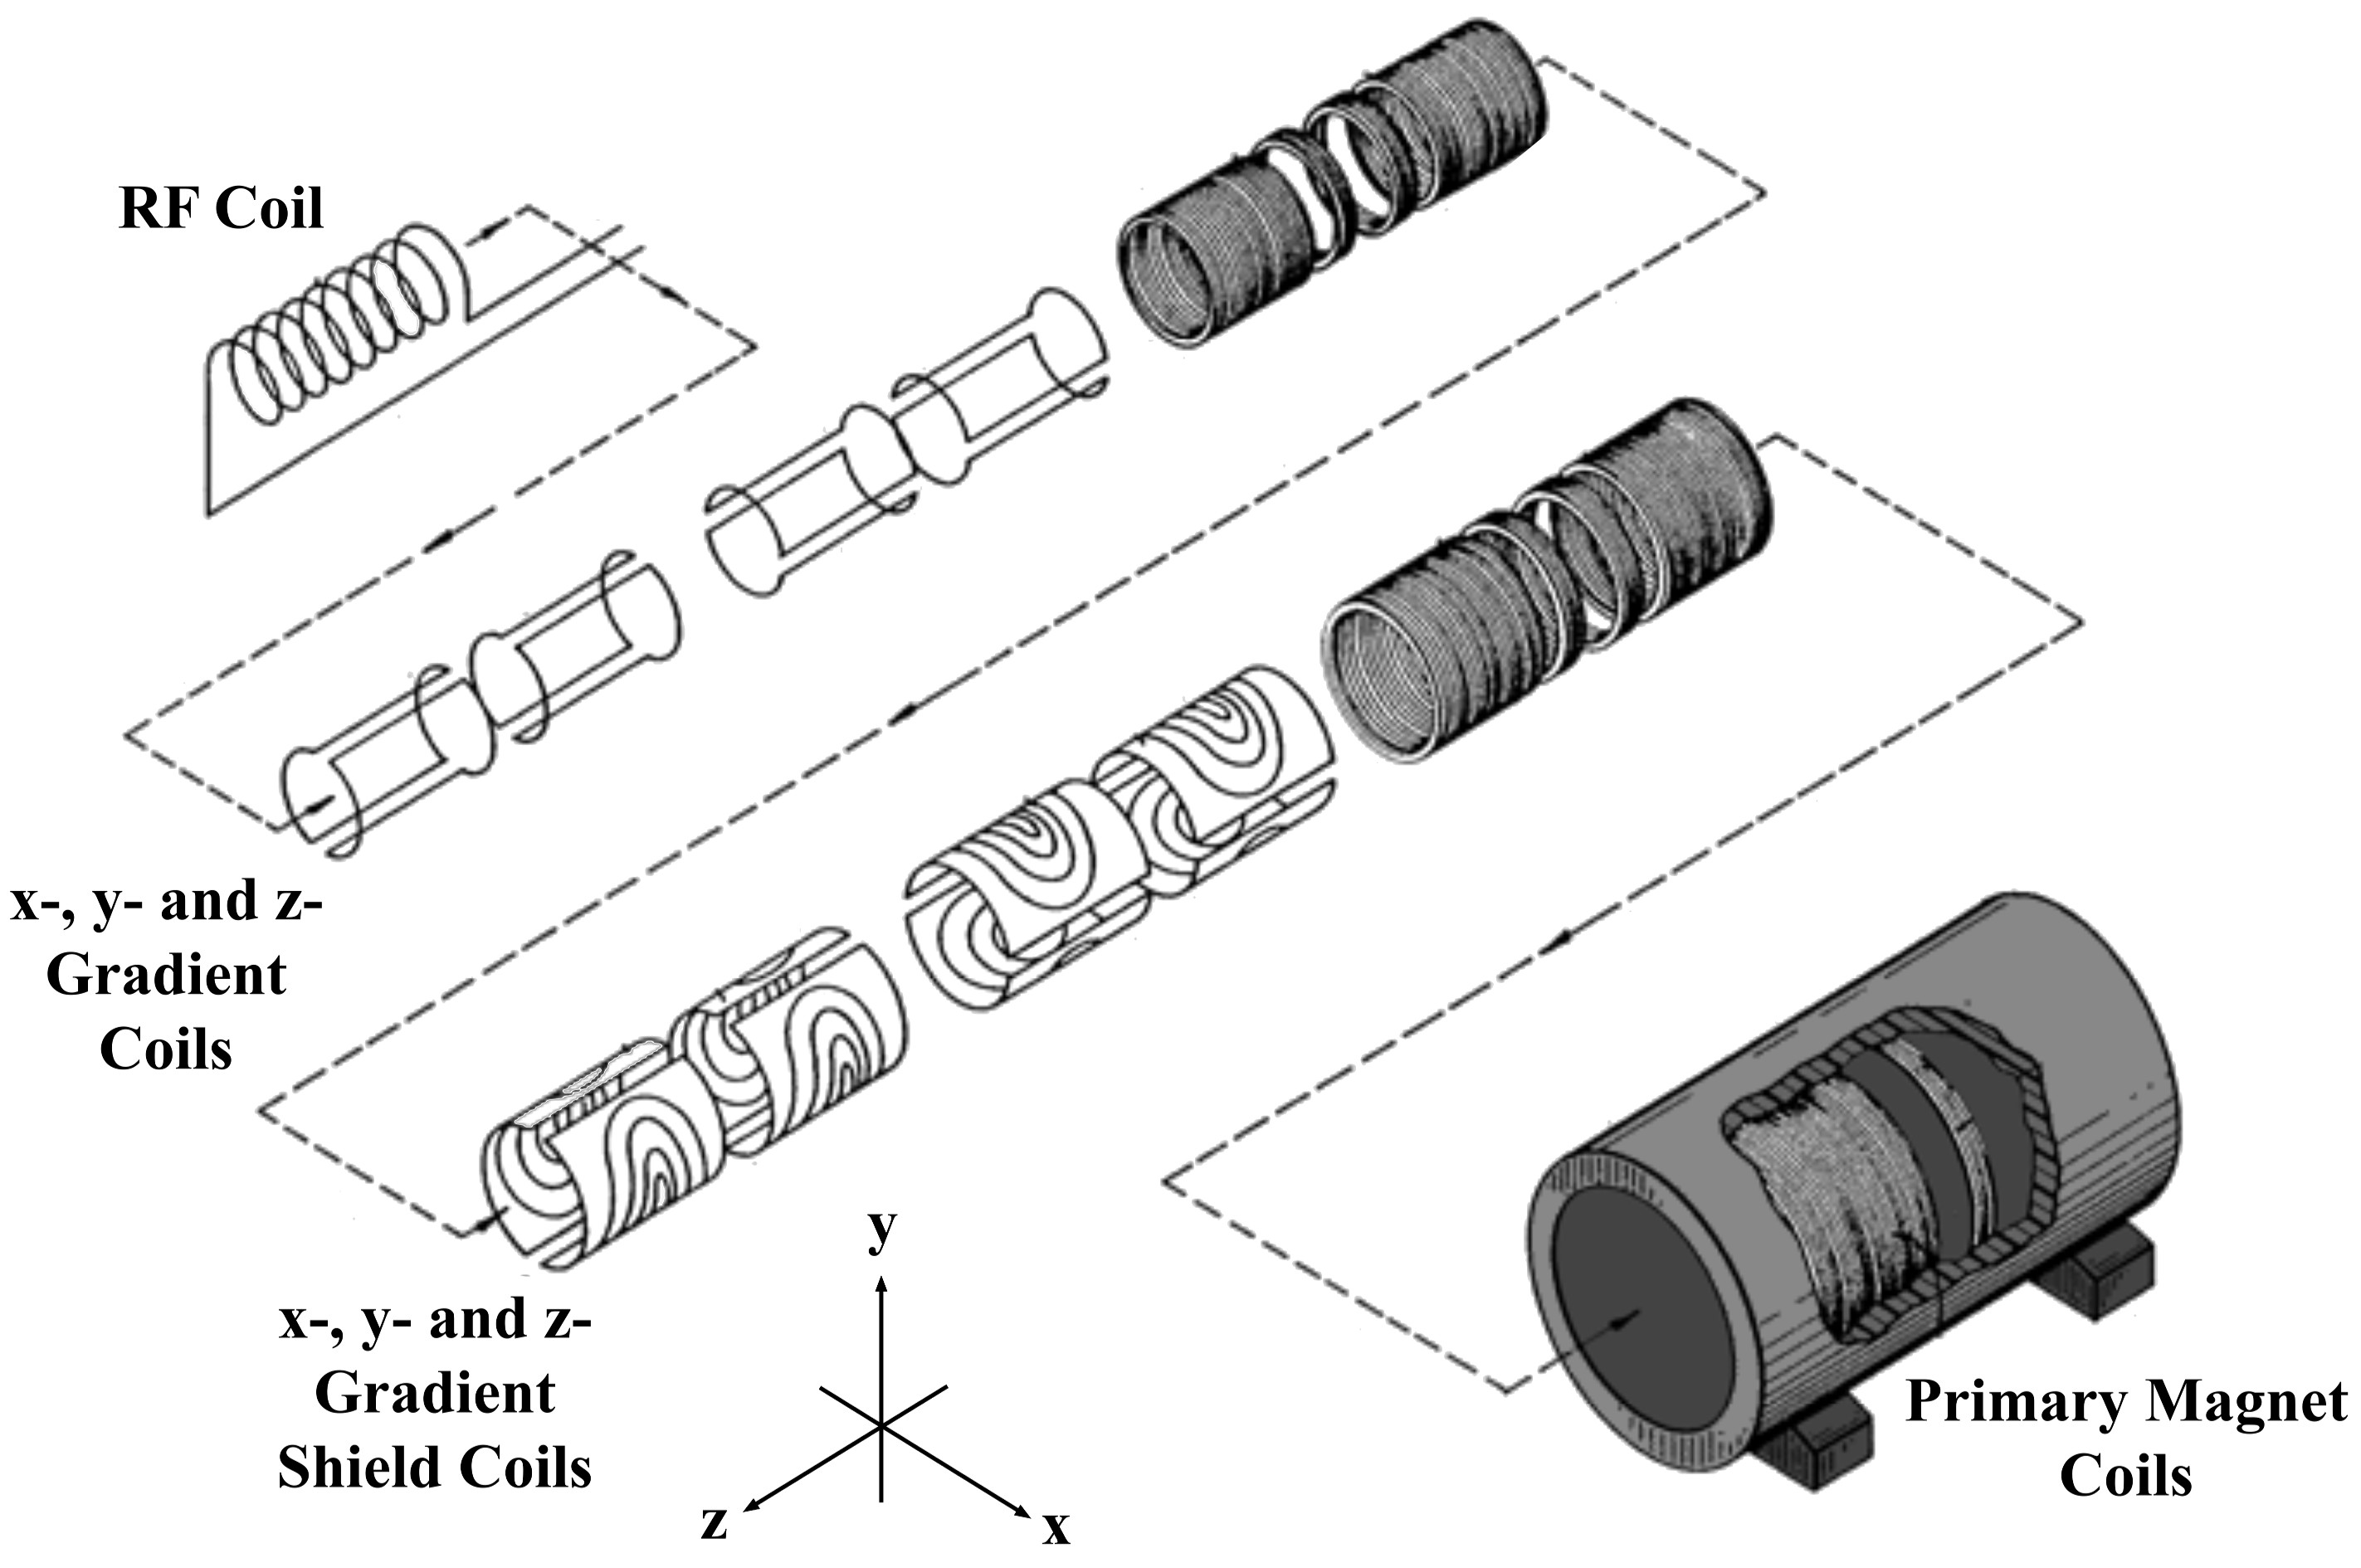
\includegraphics[width = 6cm]{./mri/pic/gradientfield.png}
%	\caption{Links die Hauptbestandteile eines MRI-Scanners und rechts die Zusammensetzung der verschiedenen Spulen \cite{MRIScanner}\cite{gradients}.}
%	\label{fig:MRIScanner}
%\end{figure}
%
%Eine wichtige Voraussetzung f"ur die Magnetresonanztomographie ist das statische Magnetfeld, welches hohe Anspr"uche erf"ullen muss. 
%Die Homogenit"at und die zeitliche Stabilit"at sind essenziell. 
%Medizinische Apparaturen arbeiten "ublicherweise mit 0.5 bis zu 3 Tesla. Neuere Ger"ate k"onnen Flussdichten bis zu 7 Tesla erreichen, daf"ur sind aber supraleitende Magnetspulen notwendig.
%
%\subsection{Das Gradientenfeld}
%
%Gem"ass Gleichung \ref{eq:larmorf} schwingen nur jene Teilchen mit $f_{Larmor}$, die der Flussdichte $B_0$ ausgesetzt sind. Um einen gew"unschten Bereich messen zu k"onnen, ist dem statischen homogenen Magnetfeld ein schw"acheres inhomogenes Gradientenfeld "uberlagert, dieses wird mit mehreren Magneten erzeugt.
%Die Gradientenfeld ist von der Position abh"angig. Ein eindimensionaler Feldgradient hat eine "Anderung das Magnetfeldes in einer Richtung. Dieser ist auch der Wichtigste.




%\subsection{Bildgebung}
%
%Es gibt verschiedene M"oglichkeiten Bilder zu generieren. Das betrifft das Messverfahren genauso wie die anschliessende Berechnung der Bilder. Eines der ersten Verfahren war \emph{Back Projection Imaging}.
%Bei diesem Verfahren wird mit einem eindimensionalen Gradientenfeld gearbeitet. Das Objekt, welches ausgemessen werden soll, wird dabei aus verschiedenen Winkeln mit dem RF-Impuls angeregt. Aus den verschiedenen Einzelmessungen kann danach ein Bild generiert werden.
%Die Bildgebung wird mit der Hilfe von Gradientenfelder bewerkstelligt. Dies sind zus"atzliche Magnetfelder, welche jeweils linear von der jeweiligen Ortskoordinaten abh"angen. Durch die "Uberlagerung des Gradientenfeldes mit dem homogenen Magnetfeld wird die Larmorfrequenz ortsabh"angig.
%\begin{equation}
%\overrightarrow{w_0} = -\gamma(\overrightarrow{B_0}+(\overrightarrow{G}\cdot \overrightarrow{r})\overrightarrow{e_x})
%\end{equation}
%\subsubsection{Ortskodierung}
%Durch HF-Impulse wird eine selektive Anregung des Spins innerhalb einer Schicht erreicht. Das Prinzip wird gleichermassen zur r"aumlichen Kodierung innerhalb der Beobachtungsschicht verwendet. Das ergibt den Auslesegradienten $G^x$, welcher die Abh"angigkeit der Resonanzfrequenz vor Ort enth"alt. Als Beispiel die Gleichung 
%entlang der $x$-Achse:
%\begin{equation}
%w_x = - \gamma G^x x
%\end{equation}

%Es gibt verschiedene M"oglichkeiten Bilder zu generieren. Das betrifft das Messverfahren genauso wie die anschliessende Berechnung der Bilder. Eines der ersten Verfahren war \emph{Back Projection Imaging}.
%Bei diesem Verfahren wird mit einem eindimensionalen Gradientenfeld gearbeitet. Das Objekt, welches ausgemessen werden soll, wird dabei aus verschiedenen Winkeln mit dem RF-Impuls angeregt. Aus den verschiedenen Einzelmessungen kann danach ein Bild generiert werden.
%
%Die Bildgebung wird mit der Hilfe von Gradientenfelder bewerkstelligt. Dies sind zus"atzliche Magnetfelder, welche jeweils linear von der jeweiligen Ortskoordinaten abh"angen. Durch die "Uberlagerung des Gradientenfeldes mit dem homogenen Magnetfeld wird die Lamaorfrequenz ortsabh"angig.
%\begin{equation}
%\overrightarrow{w_0} = -\gamma(\overrightarrow{B_0}+(\overrightarrow{G}\cdot \overrightarrow{r})\overrightarrow{e_x})
%\end{equation}
%\subsubsection{Ortskodierung}
%Durch HF-Impulse wird eine selektive Anregung des Spins innerhalb einer Schicht erreicht. Das Prinzip wird gleichermassen zur r"aumlichen Kodierung innerhalb der Beobachtungsschicht verwendet. Das ergibt den Auslesegradienten $G^x$, welcher die Abh"angigkeit der Resonanzfrequenz vor Ort enth"alt. Als Beispiel die Gleichung 
%entlang der $x$-Achse:
%\begin{equation}
%w_x = - \gamma G^x x
%\end{equation}
%>>>>>>> 929620516d75ba86c5f429616ecb9ce2ed2dde7d

\section[Quantenmechanik]{Quantenmechanik\footnote{\cite{MRI:quanten}}}
\label{sec:quant}
\rhead{Quantenmechanik}
In diesem Abschnitt wird genauer auf die quantenmechanischen Abl"aufe bei der Magnetresonanztomographie eingegangen, wobei die vorher erl"auterten Grundlagen nur ein klassisches Model sind und wenig mit der Realit"at gemein haben. Die Quantenmechanik erkl"art die realen Abl"aufe.


\subsection{Spin}
\index{Spin}
Die Grundlagen des Spins sind im Kapitel \ref{chapter:spin} erl"autert. Ein wichtiger Unterschied zur klassischen Physik ist, dass der Spin den Drehimpuls und das magnetische Moment zusammenkoppelt.

Es wird hier gezeigt, wie der Spin eines Wasserstoffatoms in einem Magnetfeld berechnet werden kann. Der daf"ur verwendete Hamilton Operator sieht f"ur ein Elektron wie folgt aus:
\begin{equation}
	H = H_0 + \frac{e}{m_e}\cdot \vec{S} \cdot \vec{B}
\end{equation}
Wobei $\vec{S}$ der Spin ist und $\vec{B}$ das Magnetfeld.

\begin{figure}
	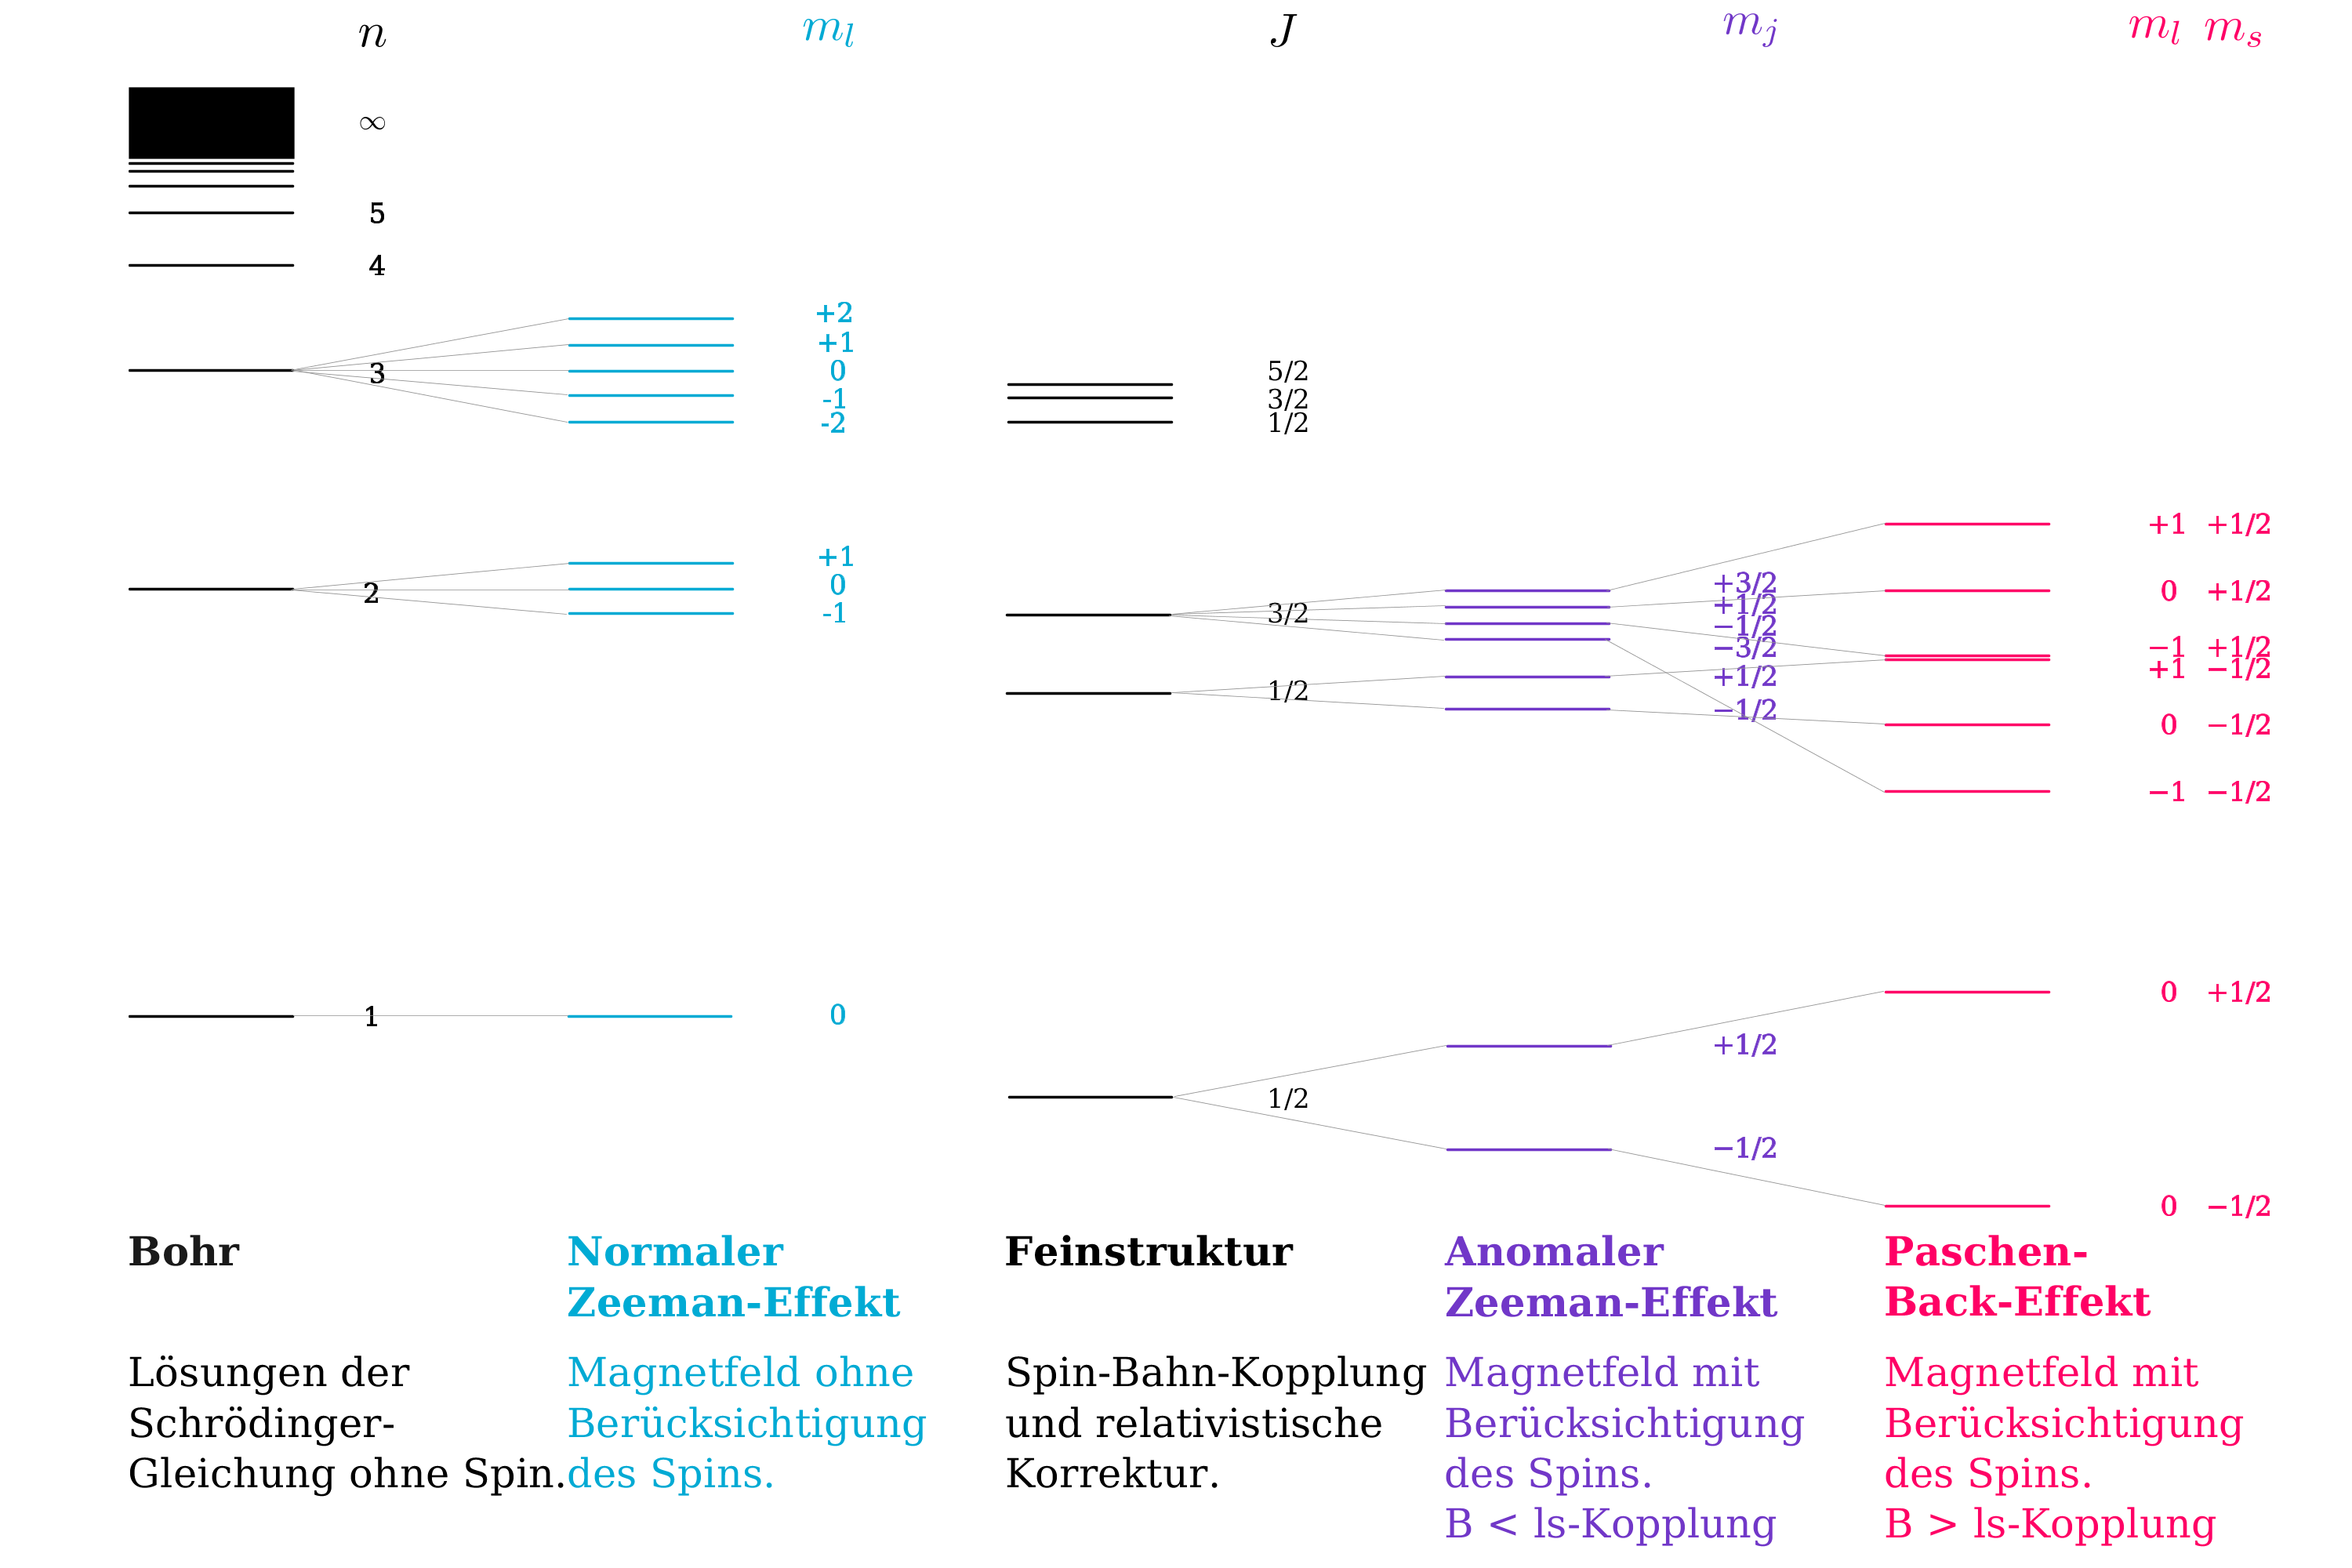
\includegraphics[width = \textwidth]{./mri/pic/index}
	\caption{Aufspaltungen der Wasserstoffniveaus unter Einfluss eines Magnetfeldes \cite{Zeeman}}
	\label{mri:quant:abb:zeeman}
\end{figure}
\index{Zeeman-Effekt}
In dem Kapitel \ref{chapter:atomuhr} wurde auf die Feinstruktur"uberg"ange eingegangen. Die Abbildung \ref{mri:quant:abb:zeeman} zeigt genau diese "Uberg"ange f"ur ein Elektron auf. Da bei der Magnetresonanztomographie aber die Protonen entscheiden sind dient die Abbildung \ref{mri:quant:abb:zeeman} nur als Veranschaulichung des Prozesses. Es wird der Hamiltonoperator f"ur ein Proton ben"otigt, dieser sieht wie folgt aus:
\begin{equation}
H = H_0 - \frac{e}{m_p }\cdot \vec{S} \cdot \vec{B}
\label{mri:hamilton}
\end{equation}
Der Term $H_0$ beschreibt den Hamiltonoperator ohne der St"orung durch ein Magnetfeld. Er stellt den Grundzustand des Protons dar. Wobei $H_0$ wie folgt definiert ist:
\begin{equation}
H_0 = \frac{\hbar}{2m_p} p^2 + V_p
\end{equation}
Bei $V_p$ handelt es sich um ein Potential, dass die Protonen im Atom an ihrem Platz h"alt.

Bei der Annahme $\vec{B} = \begin{pmatrix}
0 \\
0 \\
B_z \\
\end{pmatrix}$ ergibt sich f"ur den St"orterm $H_1$ folgende Gleichung:
\begin{equation}
H_1 = -\frac{\hbar e}{2m_p} \cdot B_z \begin{pmatrix}
1 & 0 \\
0 & -1 \\
\end{pmatrix}
\end{equation}
Aus diesem St"orterm kann nun mit der Hilfe der St"orungstheorie zwei verschiedenen Energieniveaus berechnet werden.
\index{Storungstheorie@St\"orungstheorie}
\begin{equation}
E_\downarrow^{(1)}
=
\langle \downarrow|\, H_1 \,|\downarrow\rangle
=-\frac{\hbar e}{2m_p},
\qquad
E_\uparrow^{(1)}
=
\langle \uparrow|\, H_1 \,|\uparrow\rangle
=\frac{\hbar e}{2m_p}.
\end{equation}
Der Energieunterschied ist nun also:
\begin{equation}
\Delta E = \frac{\hbar e}{m_p}B_z
\end{equation}
Der Zusammenhang mit der klassischen Physik ist nun in der Larmorfrequenz  zu finden:
\begin{equation}
\Delta E = \hbar \omega_{\text{Larmor}}=\hbar \gamma B_z
\end{equation}

\subsubsection{Einsteinsche Koeffizienten}
\index{Einstein-Koeffizienten}%
Mit der Hilfe der einsteinschen Koeffizienten kann das Prinzip wie folgt erkl"art werden.
\begin{figure}
	\centering
	%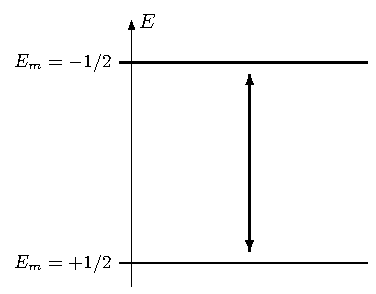
\includegraphics[width= 0.3\textwidth]{./mri/pic/einsteinischeKoeffizienten}
	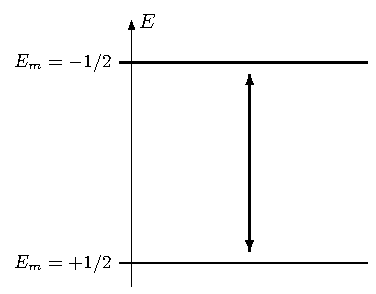
\includegraphics{./mri/pic/einsteinischeKoeffizienten}
	\caption{"Ubergang $m=+1/2 \longleftrightarrow m=-1/2$}
	\label{mri:relax}
\end{figure}
Betrachtet man die beiden Niveaus $m= -1/2$ und $m= +1/2$ in der Abbildung \ref{mri:relax} f"ur den Kernspin $1/2$ ($^1H$) so findet der einzig m"ogliche Resonanzausgleich zwischen den beiden Energieniveaus statt. 

\subsection{Zeitabh"angige Prozesse}
\index{Relaxationszeit}%
\index{Relaxationszeit!$T_1$}%
\index{Relaxationszeit!$T_2$}%
Zur Erkl"arung der vorg"angig mit der klassischen Physik erl"auterten Relaxationszeiten $T_1$ und $T_2$ werden zeitabh"angige Prozesse ben"otigt. F"ur die Relaxationszeit $T_1$ wird die zeitabh"angige Schr"odingergleichung verwendet:
\begin{equation}
\frac{\hbar}{i} \frac{\partial}{\partial x} |\psi\rangle = H\,|\psi\rangle + \text{Wechselwirkung mit der Umgebung}
\end{equation}
Wobei die zeitabh"angigen Terme folgende sind: "`Wechselwirkung mit der Umgebung"' und "'$H$"'. 
$H$ ist in der Formel \ref{mri:hamilton} ersichtlich, dabei ist der zeitabh"angige Teil im Magnetfeld $\vec{B}$ angesiedelt:
\begin{equation}
\vec{B} = \vec{B_0} + \vec{B}(t)
\end{equation}
Wobei $\vec{B}(t)$ das wechselgerichtete Magnetfeld des Hochfrequenzimpulses ist.

Bei der Wechselwirkung mit der Umgebung handelt es sich um die sogenannte Spin-Gitter-Wechselwirkung. Durch diese Wechselwirkung mit den in der Umgebung des Protons angesiedelten Atomen und Molek"ulen l"asst sich die Relaxationszeit erkl"aren. Die Zeit $T_1$ ist also nicht nur auf das Proton alleine zur"uckzuf"uhren, sondern auch auf die Atome in der Umgebung und dem Hochfrequenzimpuls.
\index{Spin-Gitter-Wechselwirkung}%
\index{Relaxationszeit!longitudinal}

\subsubsection{Relaxationszeit $T_2$}
Die Transversale  Relaxationszeit $T_2$ wird bestimmt durch statistische Gegebenheiten der Protonen. Das heisst, dass die Zeiten mehrerer Protonen ausgewertet werden. Mit der Theorie in diesem Skript kann die Relaxationszeit $T_2$ nicht beschrieben werden. Dazu w"are die Quantenmechanik mehrerer wechselwirkender Teilchen notwendig. 
\index{Relaxationszeit!transversal}

Zur Veranschaulichung zeigt die Tabelle \ref{mri:quant:tab:zeiten} einige Relaxationszeiten f"ur verschiedene Gewebearten.

\begin{table}
	\centering
		\begin{tabular}{|l|c|c|}
			\hline
			Gewebeart & $T_1$ (ms) & $T_2$ (ms) \\
			\hline
			Lunge & 830 & 79 \\
			Leber & 490 & 43 \\
			Milz & 780 & 67 \\
			Niere & 650 & 58 \\
			Fett & 260 & 84 \\	
			\hline	
		\end{tabular}
		\caption{Unterschiedliche Relaxationszeiten verschiedener
			Gewebearten bei $|\vec{B}|$ = 1.5 T}
		\label{mri:quant:tab:zeiten}
\end{table}
%TODO Relaxation T_1
%TODO relaxation durch spin-lattice-relaxtion erklären -> Durch die umgebungsatome und deren Feldern wird die Relaxationszeit T_1 beeinflusst sprich definiert.
%
%Zeitabhänigge Schrödinger gleichung aufzeichnen
%Relaxtion T_2 ist zu wenig bekannt es handelt sich um eine statistische berechnung.
%TODO EIne statistische 









%Alle Atome mit einer ungeraden Anzahl von Protonen und/oder Neutronen (z.B. 
%$^1
%H, 
%^13
%C$) besitzen in ihrem Grundzustand einen von Null verschiedenen Kernspin. 
%%Damit ist das Dipolmoment gegeben durch
%%\begin{equation}
%%\vec{\mu}=\gamma \vec{S} = \gamma H \vec{S}
%%\end{equation}
%Ist ein solches kernmagnetisches Moment im Magnetfeld vorhanden, so beobachtet man den Zeeman Effekt. Dieser "aussert sich durch die Aufspaltung der Spektrallinien wie es in der Abbildung \ref{mri:quant:abb:zeeman} ersichtlich ist. In einer ersten N"aherung kann dieser Effekt durch ein ungest"orter, nicht relativistischen Hamilton Operator erkl"art werden. F"ur ein konstantes Magnetfeld in $z$-Richtung sieht dieser wie folgt aus:
%\begin{equation}
%H_{0,z} = -\gamma \vec{B} \vec{S}
%\end{equation}
%
%
%\subsection{Relaxation}
%Unter Relaxation versteht man die Vorg"ange, welche die Kernspin-Magnetisierung in ihren Gleichgewichtszustand zur"uckkehren l"asst, dass ergibt unterschiedliche Relaxationzeiten, welche f"ur die Bildgebung verwendet werden k"onnen. Unterschiedliche Gewebearten ergeben verschiedene Zeiten. Die Tabelle \ref{mri:quant:tab:zeiten} stellt einige Zeiten dar.
%\begin{table}
%	\centering
%		\begin{tabular}{|l|l|l|}
%			\hline
%			(bei B = 1.5 T) & $T_1$ (ms) & $T_2$ (ms) \\
%			\hline
%			Lunge & 830 & 79 \\
%			Leber & 490 & 43 \\
%			Milz & 780 & 67 \\
%			Niere & 650 & 58 \\
%			Fett & 260 & 84 \\	
%			\hline	
%		\end{tabular}
%		\caption{Unterschiedliche Relaxationszeiten verschiedener Gewebearten}
%		\label{mri:quant:tab:zeiten}
%\end{table}
%
%\subsubsection{Prinzip}
%Bei einem Gleichgewicht im Magnetfeld ist die Kernmagnetisierung $\vec{M} = M_0\vec{e_z}$ entlang der Feldrichtung. Die Gr"osse $M_0$ ist durch die Boltzmann-Statistik definiert. Die Magnetiesierungskomponente in $z$-Richtung nennt man longitudinale Magnetisierung. Die Magnetisierungskomponenten in $x$- und $y$-Richtung sind im Gleichgewichtsfall in ihrem Betrag gleich null. Durch eine Einstrahlung eines Hochfrequenzimpulses, wird die $z$-Komponente der Magnetisierung $M_z$ gleich null (bzw. -$M_0$). Zus"atzlich ensteht durch diese St"orung auch ein Kernmagnetisierung in $x$-$y$-Ebene mit dem Betrag $M_\perp \neq M_0$. Die Abbildung \ref{mri:quant:abb:Relaxionszeiten} stellt dies grafisch dar.
%\begin{figure}[h]
%	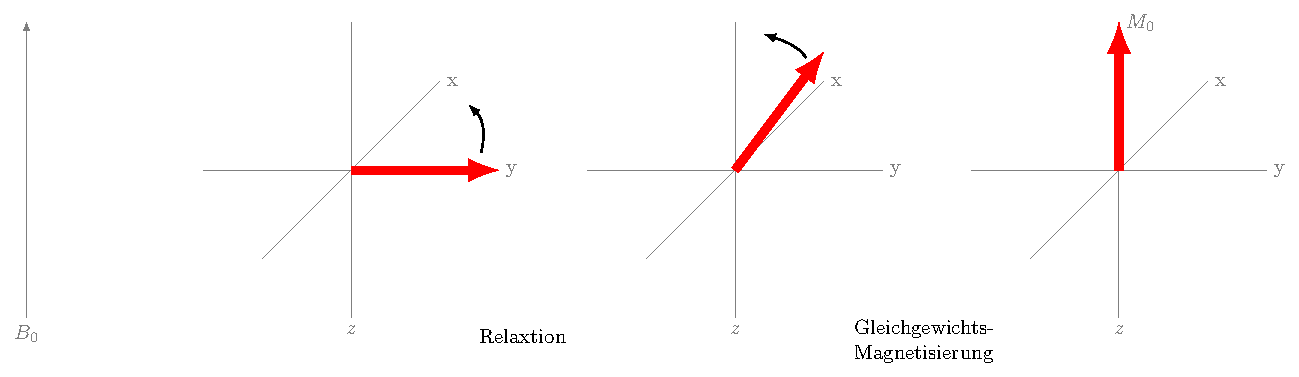
\includegraphics[width= \textwidth]{./mri/pic/relax}
%	\caption{Relaxionszeiten}
%	\label{mri:quant:abb:Relaxionszeiten}
%\end{figure}

%F"ur die Larmorfrequenz der Kernresonanz gilt zumindest oberhalb der Temperatur von einem Kelvin $h v \ll kT$. Deshalb k"onnen die spontanen "Uberg"ange 
%vernachl"assigt werden, und die Wahrscheinlichkeiten f"ur Absorption und induzierte Emission 
%sind gleich.



%\subsubsection{Longitudinale Relaxationszeit $T_1$}
%Die Longitudinale Relaxationszeit ist durch die Zeit $T_1$ definiert. Diese ist definiert durch die Zeit, welche das gest"orte System ben"otigt um in den Gleichgewichtszustand zur"uckzukehren. Dies wird dadurch erreicht, dass das System an die Umgebung Energie verliert.
%\begin{figure}[H]
%\caption{Longitudinale Relaxationszeit $T_1$}
%\label{mri:quant:abb:long}
%\end{figure}

%\subsubsection{Transversale  Relaxationszeit $T_2$}
%Die transversale Relaxationszeit ist durch die Zeit $T_2$ definiert. Sie beschreibt das zeitliche Verhalten der Magnetisierung in der $x$-$y$-Ebene. 
%\begin{figure}[H]
%	\caption{Transversale Relaxationszeit $T_1$}
%	\label{mri:quant:abb:trans}
%\end{figure}


\section{Anwendung ausserhalb der Medizin \label{chapter:MRI:bsp}}

Im folgenden Abschnitt wird die Anwendung des Prinzips ausserhalb der Medizin erl"autert. Er unterteilt sich in die beiden Unterkapitel "`Wasserstoff als Signalgenerator"' und "`NMR-Spektrum"'. Die theoretischen Grundlagen zu diesem Kapitel wurden im Kapitel\;\ref{sec:quant} erl"autert.

\subsection{Wasserstoff als Signalgenerator}
Die Motivation war herauszufinden, ob es m"oglich ist, Fossilien in einem Stein zu erkennen. Die Problematik in diesem Fall ist, dass es sich um Materialien handelt, die arm an Wasserstoffatomen sind, welche f"ur die Bildgebung eine massgebende Rolle spielen. Wie in Tabelle\;\ref{mri:bsp:tab:NMR_Kerne} ersichtlich, ist das abgegebene Signal der Nicht-Wasserstoffatome massiv geringer. Aus diesem Grund werden nur H-Atome benutzt, um MRI Bilder zu generieren. Daraus folgt, dass das MRI nicht geeignet ist zur Erzeugung von Bildern im Stein verborgener Knochen. Es ist zwar heutzutage m"oglich 3D-Bilder vom Inneren eines Steines zu machen, jedoch nutzen alle Ger"ate R"ontgenstrahlen, welche ohne Hilfe des Kernspins auskommen.
\begin{table}[h]
	\centering
	\begin{tabular}{|c|c|c|c|}
		\hline
		Kern 				& $\omega_0$ 	& Relative 				& Relatives\\
							& @ 1.5T [MHz] 	& Signal-Intensit"at 	& Gesamt Signal\\
		\hline
		$\mathrm{^{1}H}$ 	& 63.8 			& 1.000 				& 1.000 \\
		$\mathrm{^{13}C}$ 	& 16.1 			& 0.016 				& 0.0000001 \\
		$\mathrm{^{19}F}$ 	& 60.1 			& 0.833 				& 0.000001 \\
		$\mathrm{^{31}P}$ 	& 25.8 			& 0.066 				& 0.00001 \\
		\hline
	\end{tabular}
	\caption{Relative Empfindlichkeit einiger NMR-Kerne \cite{skript:mri:AMSM_Paper}}
	\label{mri:bsp:tab:NMR_Kerne}
\end{table}
Doch weshalb ist das Signal der Wasserstoffatome so viel klarer und st"arker als die Signale der anderen Atome? Bei genauerer Betrachtung der Tabelle\;\ref{mri:bsp:tab:NMR_Kerne} l"asst sich feststellen, dass die relative Signal-Intensit"at des "`Fluor 19"' Atoms der des Wasserstoff Atoms am n"achsten kommt. Wenn man davon ausgehen darf, dass Kerne "ahnlich wie Atome eine Schalenstruktur aufweisen, dann hat Fluor-19 wahrscheinlich eine ziemlich spezielle Struktur, weil sich mit 18 Nukleonen eine stabile Konfiguration erzielen l"asst -- ebenso wie mit 18 Elektronen (bei Argon). Das 19. Nukleon ist daher in einer neuen Schale relativ exponiert, und d"urfte sich "ahnlich wie das nackte Proton eines Wasserstoffkerns verhalten. Da Fluor im Vergleich zum Wasserstoff relativ selten auf der Erdkruste und erst recht in Menschen oder Tieren vorhanden ist, stellen sich die H-Atome als perfekte Signalgeneratoren dar und "uberbieten die F-Atome. 

\subsection{NMR-Spektrum}
Obwohl das Prinzip des MRI ausserhalb der Medizin keinen grossen Anklang fand, wird in einigen Labors diese Methode zur Analyse von Stoffen genutzt. Die meist von Chemikern eingesetzte Maschine -- der eigentliche Vorg"anger des MRIs -- ist unter dem Namen NMR-Spektrometer bekannt. Dieser arbeitet mit Feldern von bis zu 21 Tesla, was im Vergleich zur Medizin, die typischerweise MRI-Ger"ate einsetzt, welche Felder zwischen 0.5 und 3 Tesla\footnote{Ein paar wenige Kliniken besitzen MRI-Ger"ate mit 7 - 9 Tesla} generieren, um einiges st"arker ist. Das Feld bei einer Kernspinresonanzspektroskopie, kurz NMR-Spektroskopie (von der englischen Bezeichnung ”nuclear magnetic resonance“), wird meistens in einem Loch von der Gr"osse eines Reagenzglases erzeugt. Ein Beispiel eines solchen Ger"ats ist auf der Abbildung\;\ref{mri:bsp:abb:nmr_Beispiel} zu sehen. 
\begin{figure}[h]
	\centering
	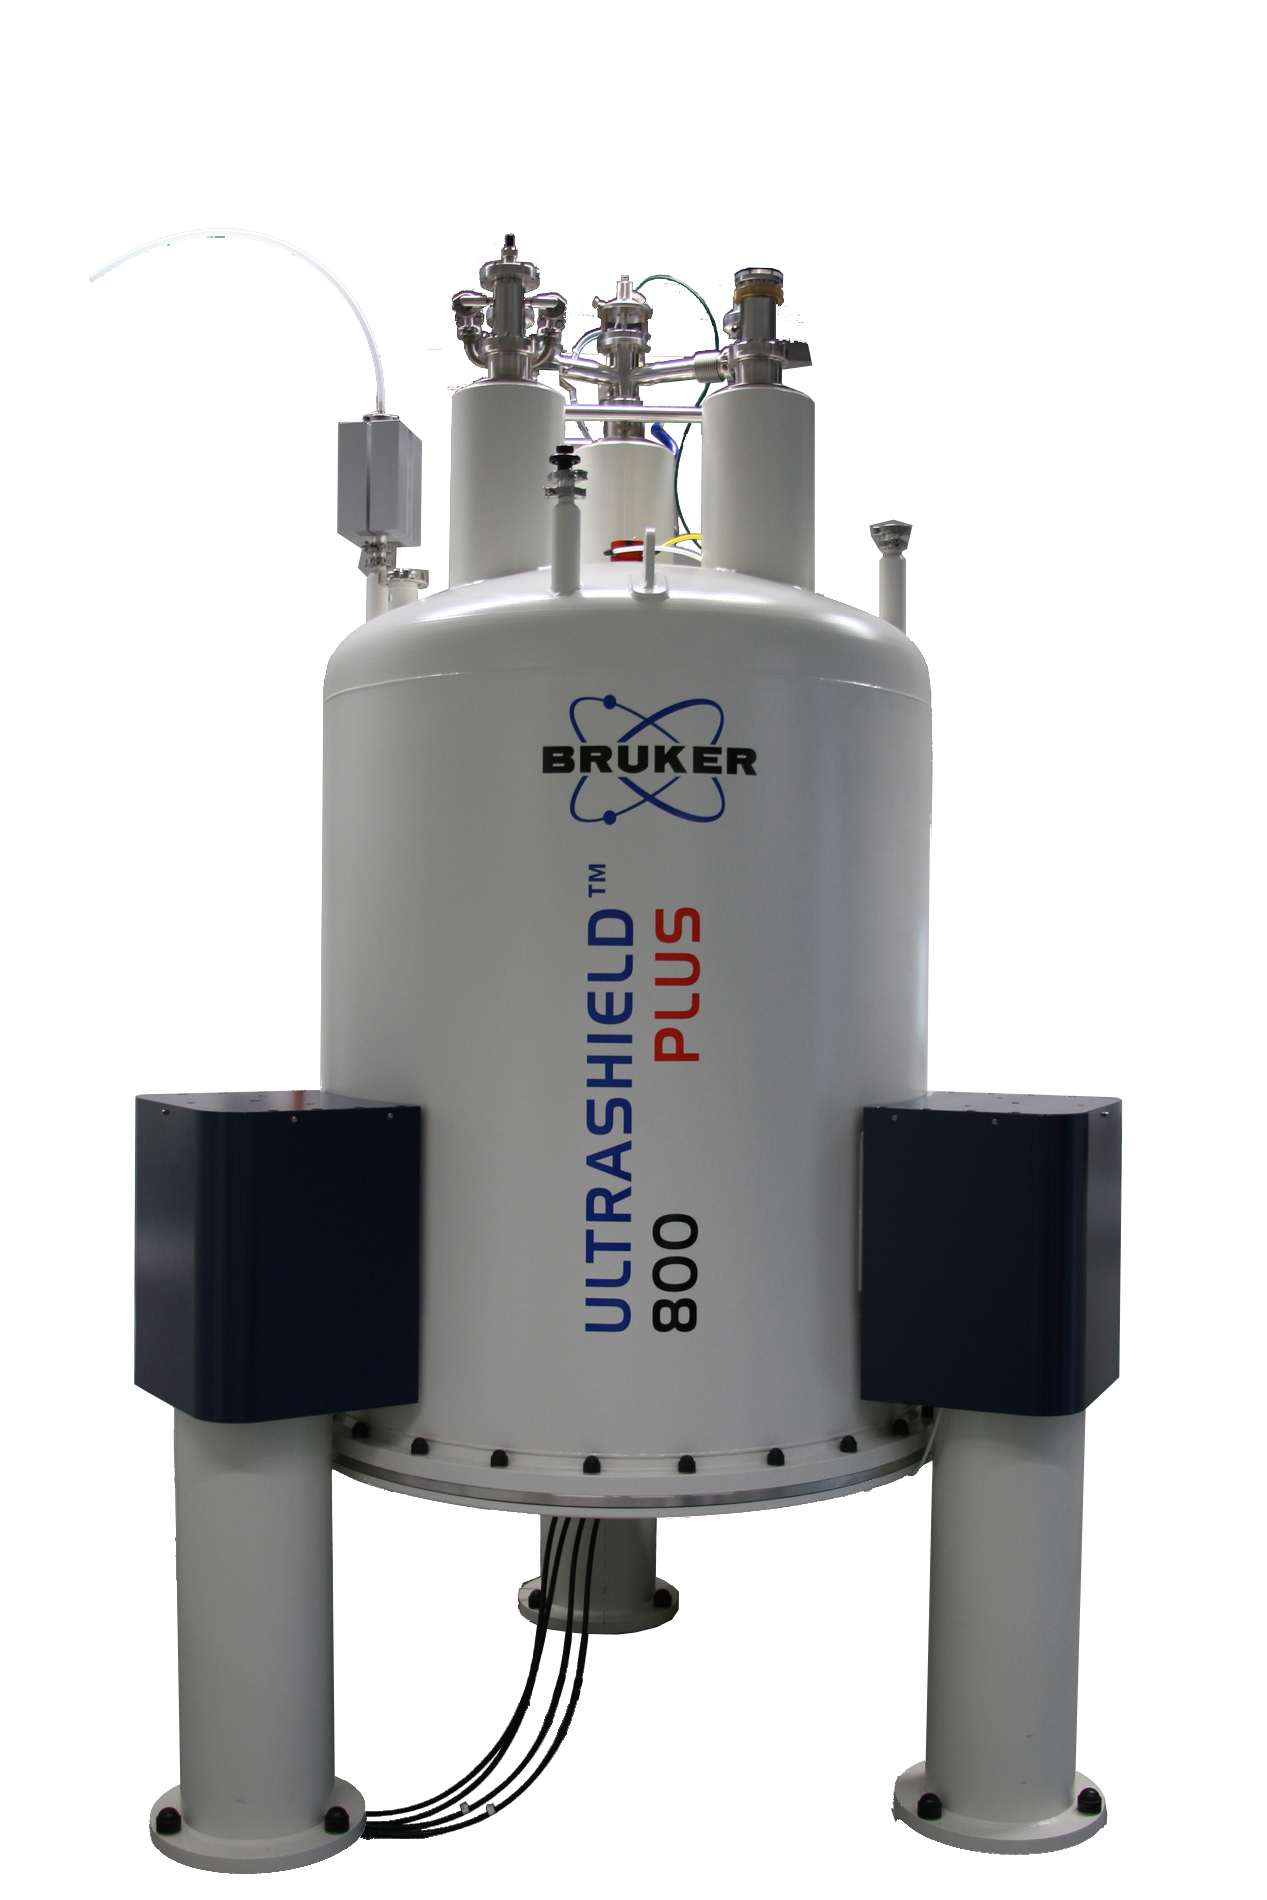
\includegraphics[width = 3cm]{./mri/pic/NMR.png}
	\caption{Beispiel eines NMR-Ger"ates \cite{skript:mri:MaxPlanckCampus}}
	\label{mri:bsp:abb:nmr_Beispiel}
\end{figure}

\subsubsection{Bildausgabe}
Das Bild, welches bei einem NMR-Spektrometer entsteht, sieht nicht etwa so aus wie das eines MRI (siehe Abbildung \ref{mri:abb:kiwi} / \ref{mri:abb:ananas}), sondern gibt ein Spektrum wieder. Die Abbildung\;\ref{mri:bsp:abb:Etanolspektrum} zeigt eines der ersten NMR-Spektren, f"ur welches Edward Mills Purcell zusammen mit Felix Bloch 1952 den Nobelpreis f"ur Physik bekamen. Im aktuellen NMR-Spektren ist die Abszisse gespiegelt, d.h. sie geht von tieferen zu h"oheren Frequenzen. Was auf dieser Spektrum direkt zu sehen ist, sind die drei verschieden hohen Signale, welches vom NMR aufgenommen wurden. Das h"ochste Signal geh"ort dem $\mathrm{CH_3}$-Teil des Molek"uls, da dieser Molek"ul-Abschnitt die meisten H-Atome besitzt und somit das h"ochste magnetische Potenzial. Analog dazu lassen sich die zwei weiteren Ausschl"age des $\mathrm{CH_2}$- und OH-Teiles zu interpretieren. 
\begin{figure}[h]
	\centering
	\begin{minipage}{0.55\textwidth}
		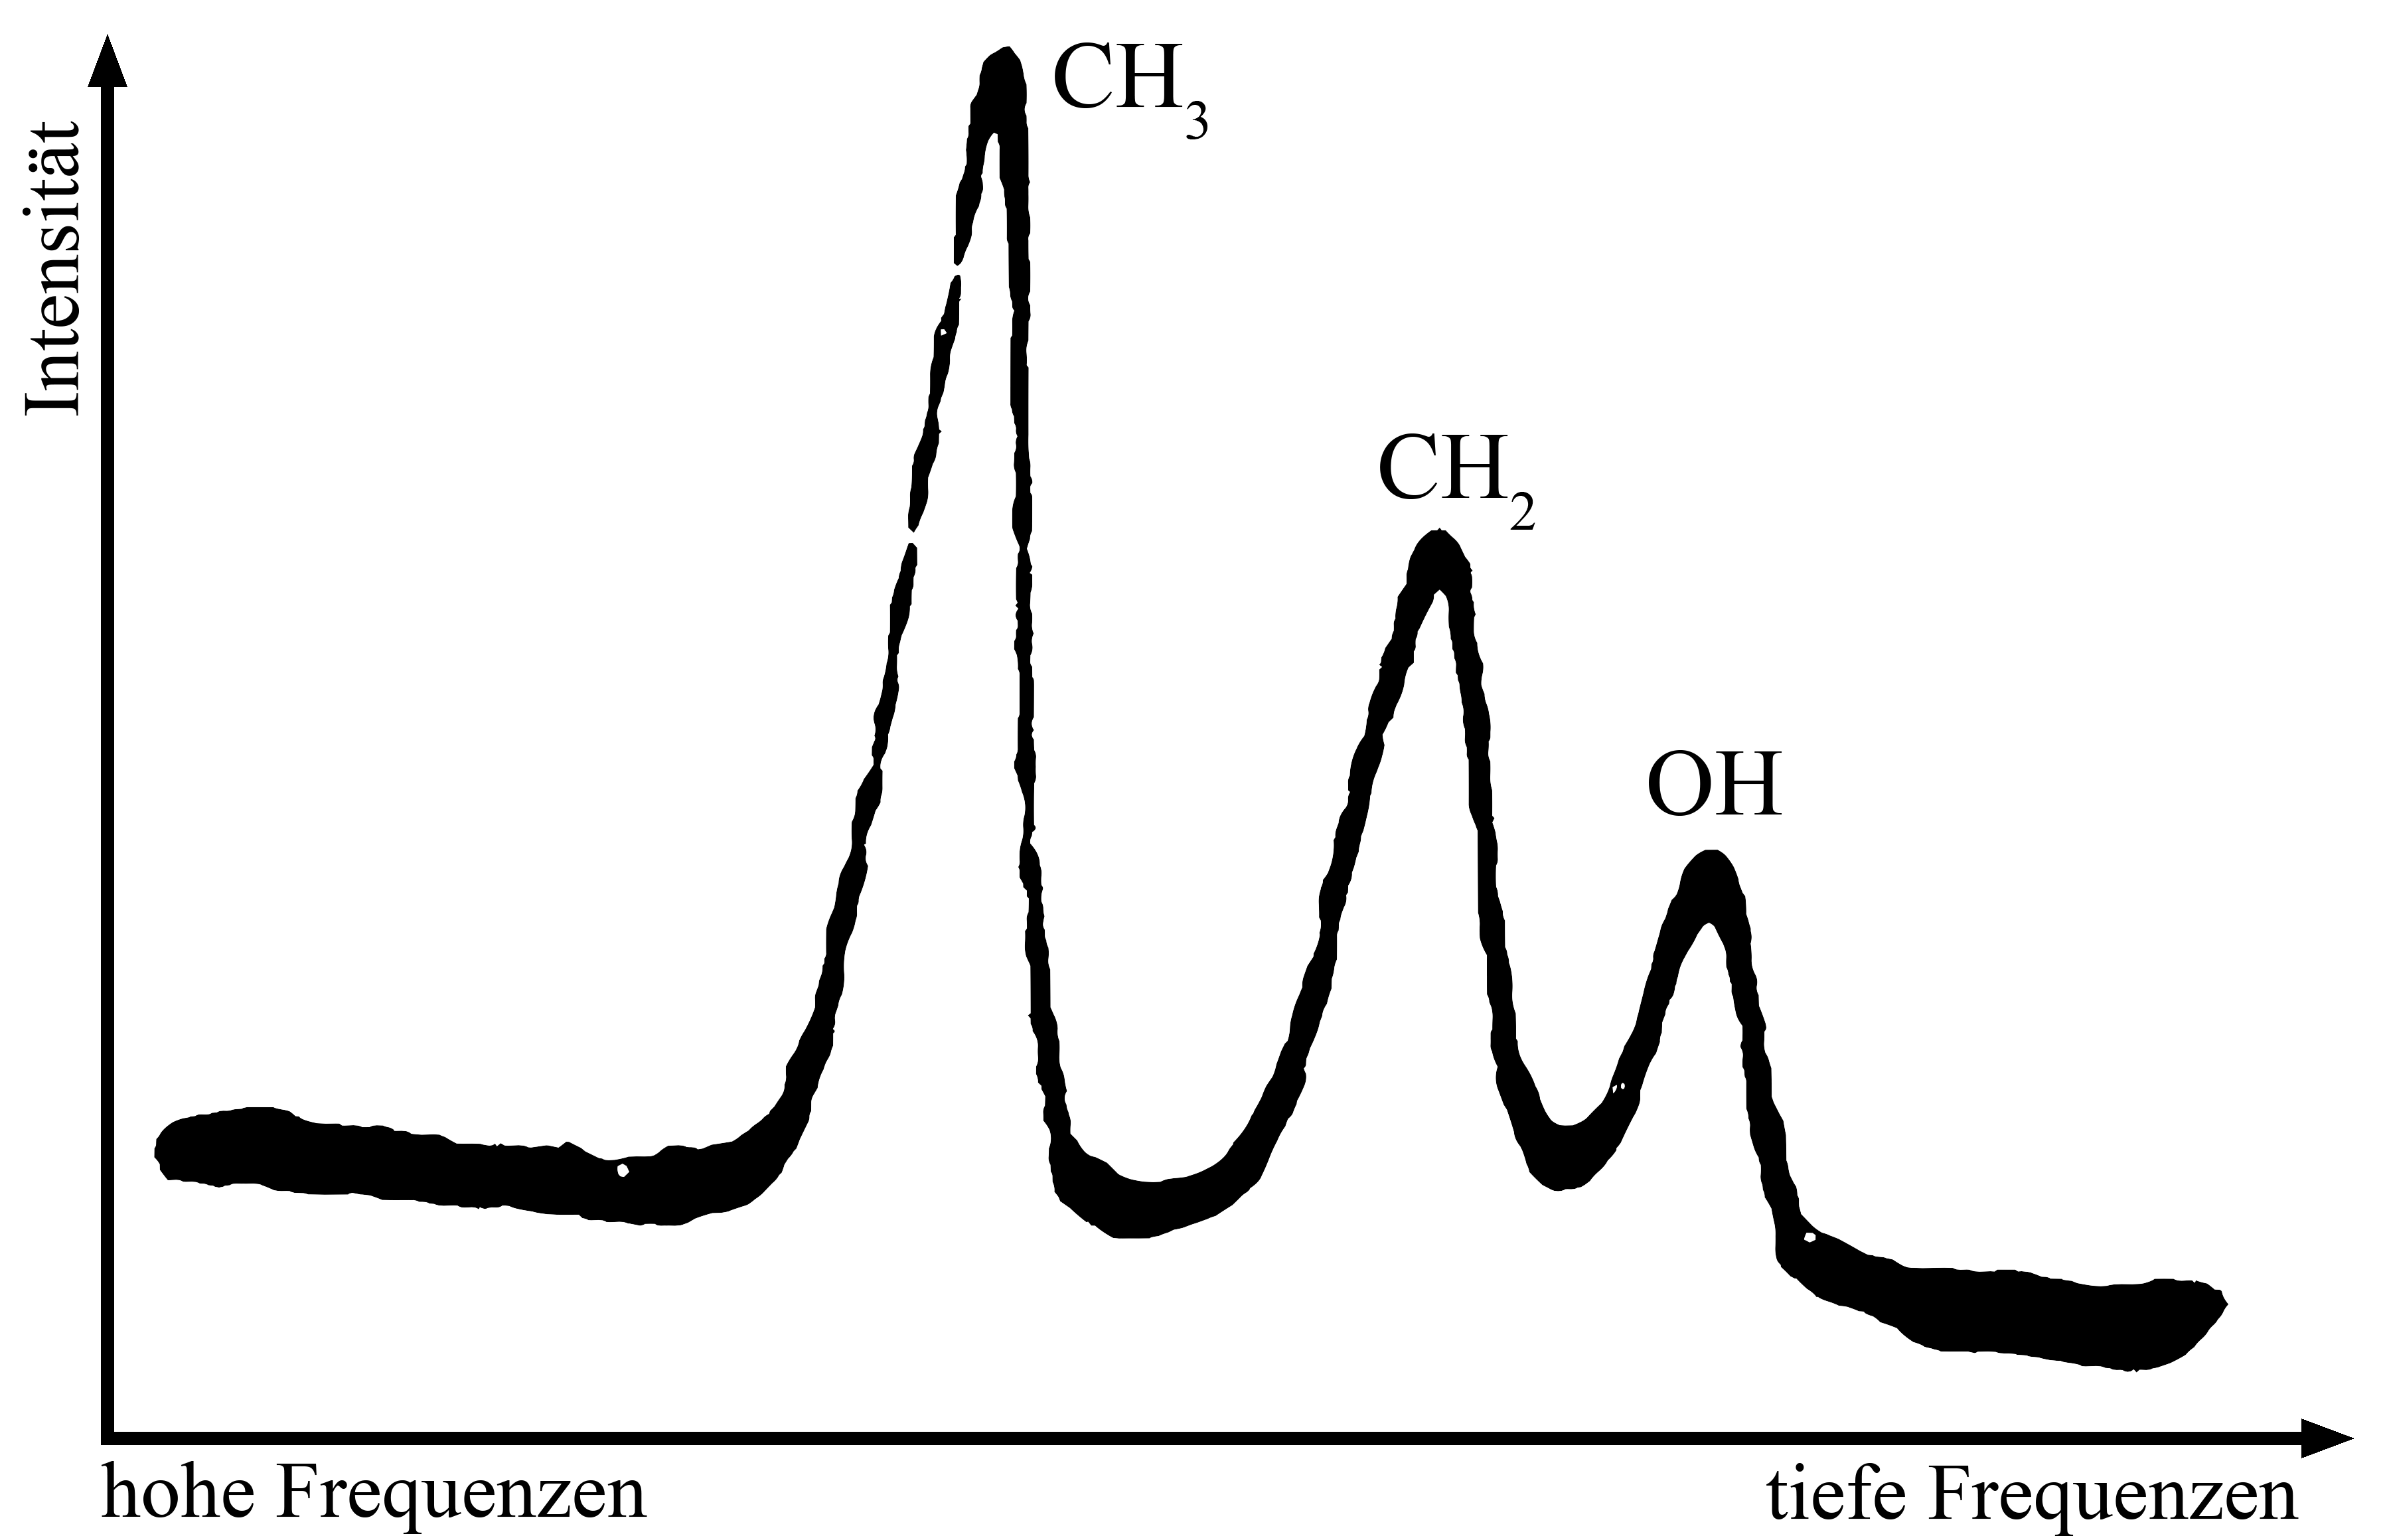
\includegraphics[width = \textwidth]{./mri/pic/CW_SpektrumEthanol.png}
	\end{minipage}
	\begin{minipage}{0.42\textwidth}
		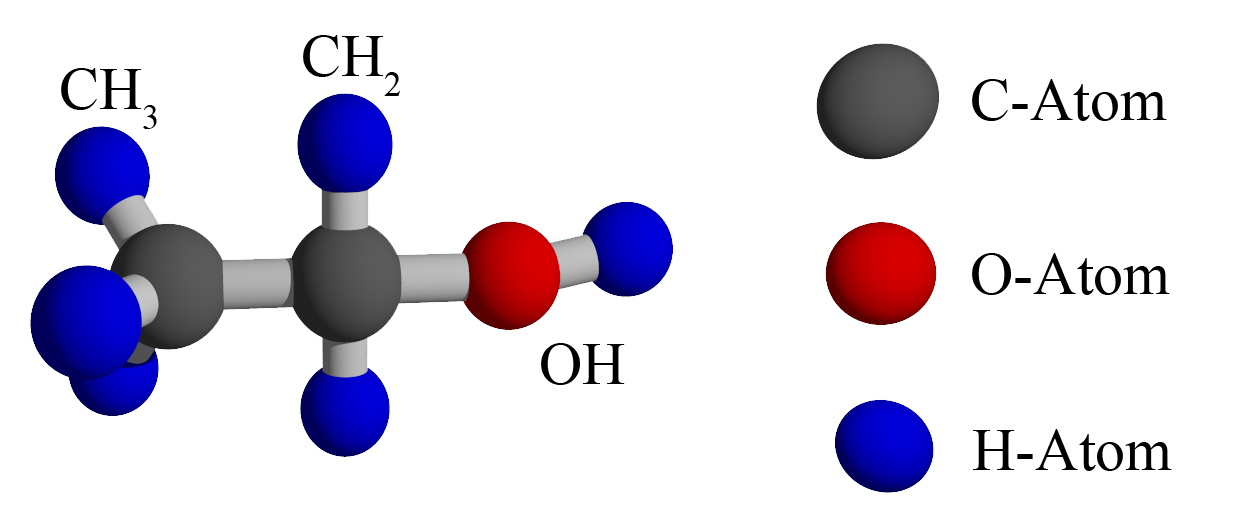
\includegraphics[width = \textwidth]{./mri/pic/Ethanol.png}
	\end{minipage}
	\caption{Ethanol NMR-Spektrum \cite{skript:mri:NMRSkopie} und ein Ethanolmolek"ul}
	\label{mri:bsp:abb:Etanolspektrum}
\end{figure}
Die Verschiebung der Frequenz (Abweichung auf der $x$-Achse) ist schwieriger zu verstehen, da es sich hier um Wasserstoffatome handelt, die das Signal abgeben. Diese geben wiederum -- wie in Tabelle\;\ref{mri:bsp:tab:NMR_Kerne} ersichtlich -- immer bei der gleichen Frequenz Signale ab. In der Chemie, wo auch die meisten NMR-Ger"ate eingesetzt werden, wird f"ur dieses Ph"anomen das Sauerstoff-Atom verantwortlich gemacht. Bei diesem Atom handelt es sich um ein elektronengieriges, d.h. dass dieses die Elektronen des direkt angeschlossenen Wasserstoffatomes stark anzieht und somit eine Art Abschirmung gegen aussen erzeugt, was wiederum die Frequenz beeinflusst. Die zwei Wasserstoff-Atome des $\mathrm{CH_2}$-Teils hingegen sind "uber das Kohlenstoff-Atom etwas abgekoppelt. Nichts desto trotz k"onnen sie den Einfluss des O-Atoms immer noch sp"uren, w"ahrend die H-Atome des $\mathrm{CH_3}$-Teiles fast nichts mehr vom Sauerstoff-Atom mitbekommen. Die Chemiker nennen es eine Elektronen Wolke, die um das O-Atom entsteht, welche wiederum wie ein Schild wirkt.

\subsubsection{Heutiger Einsatz in der Chemie}
Die Abbildung \ref{mri:bsp:abb:EtanolspektrumNew} zeigt ein aktuelles Spektrum des Ethanols. Dieses genauer zu erkl"aren w"urde jedoch den Rahmen dieses Artikels sprengen, denn hier sind bereits die Kopplungen der H-Atomen zu den benachbarten Segmenten herauslesen. Was aber deutlich zu erkennen ist, ist die feinere Aufl"osung. Dank des Fortschritts, welcher bis jetzt gemacht werden konnte, erlauben diese NMR-Spektren den Chemikern Stoffe bis in die molekulare Ebene zu untersuchen und zu bestimmen. 
\begin{figure}[h]
	\centering
	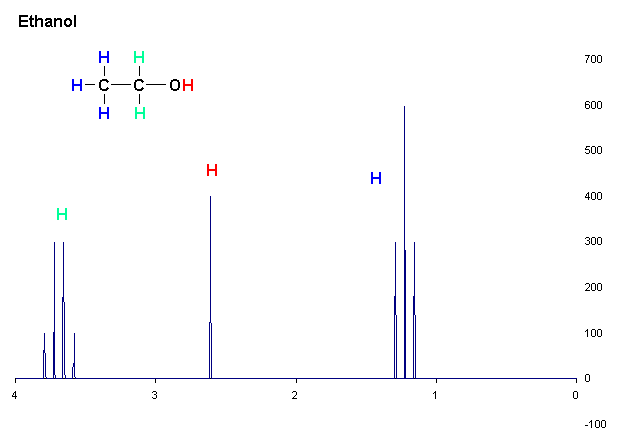
\includegraphics[width = 0.75\textwidth]{./mri/pic/CW_SpektrumEthanol_Neu.png}
	\caption{Aktuelles Ethanol NMR-Spektrum \cite{skript:mri:EthanolNeu}}
	\label{mri:bsp:abb:EtanolspektrumNew}
\end{figure}